\chapter{Analysis}
\begin{chapterabstract}
This chapter covers the~analysis of current gaze tracking practises, systems implementing ET, the~latest VR devices with ET and the~capabilities of Unreal Engine with possibilities of implementing ET in it.
\end{chapterabstract}

\section{Gaze tracking}

ET technology combined with VR allows one to~estimate the~gaze direction in a~3D world, which is a~3D vector. Various techniques that solve the~manipulation, classification, and storage of this line of sight are part of gaze tracking.

\subsection{Fundamentals}
The~way an~eye moves can be described as a~continuous sequence of two alternating actions;~fixation and saccade.~\cite{hansen2010, anuradha2017review}

\begin{description}
    \item[Fixation] is a~stable but non-static gaze state that rests on a~small area for a~period of time. A~gaze can only be classified as a~fixation if it remains in the~area for a~defined minimum threshold duration -- usually 80~ms.
    \item[Saccade] is a~gaze state that indicates rapid movements of the~eye between fixations. It can be classified as such if the~gaze leaves the~small area prior to fixation classification.
\end{description}


Fixation is the~main metric used in ET, but it requires context. In order to~use gaze to~determine fixation within a~3D scene, it is first necessary to~segment the~scene into several logical sections.


\subsubsection*{Region of Interest}
This segment is called \emph{Region of Interest} (RoI), which provides the~context for the~fixation, i.e., the~gaze target. These can be defined as large areas with multiple objects or, alternatively, as small details. Each virtual scene contains information about its objects and their absolute positions in its coordinates. It is reasonable to~create RoIs according to~individual objects in a~given scene.~\cite{ugwitz2020thesis}

An~ET experiment consists of subtasks during which fixations and saccades at different RoIs are captured over time to~determine when and where the~subject gazed at. This information can be used in the~creation of further structures that provide more context to the~subject's behaviour during an~experiment.~\cite{koenig2019}

\subsubsection*{Scanpath}
One of these is \emph{scanpath}~\cite{anuradha2017review}, which consists of an~alternating sequence of fixations and saccades. These are not only useful for storing the~sequence of eye movements over time, but also can be used to~infer the~duration and distance between two different fixations.

With its combination, more precise information is obtained about each \emph{region of interest}, from which one can infer how much time elapsed before the~first fixation in the~RoI or how many and which regions were visited before. Another related metric is \emph{gaze duration}, which sums the~duration of all fixations in a~single RoI.

\subsection{Gaze data}
\label{sec:gaze-data}
The~data are constructed in real time during the~experiment or after its end. Everything depends on the~deployed hardware. It is recommended to have all available performance ready to~use for the~experiment itself. For later processing of ET data, it is crucial to~record the~gaze data first. Sources used for this section~\cite{ugwitz2020thesis, koenig2019}

\begin{figure}[!ht]\centering
    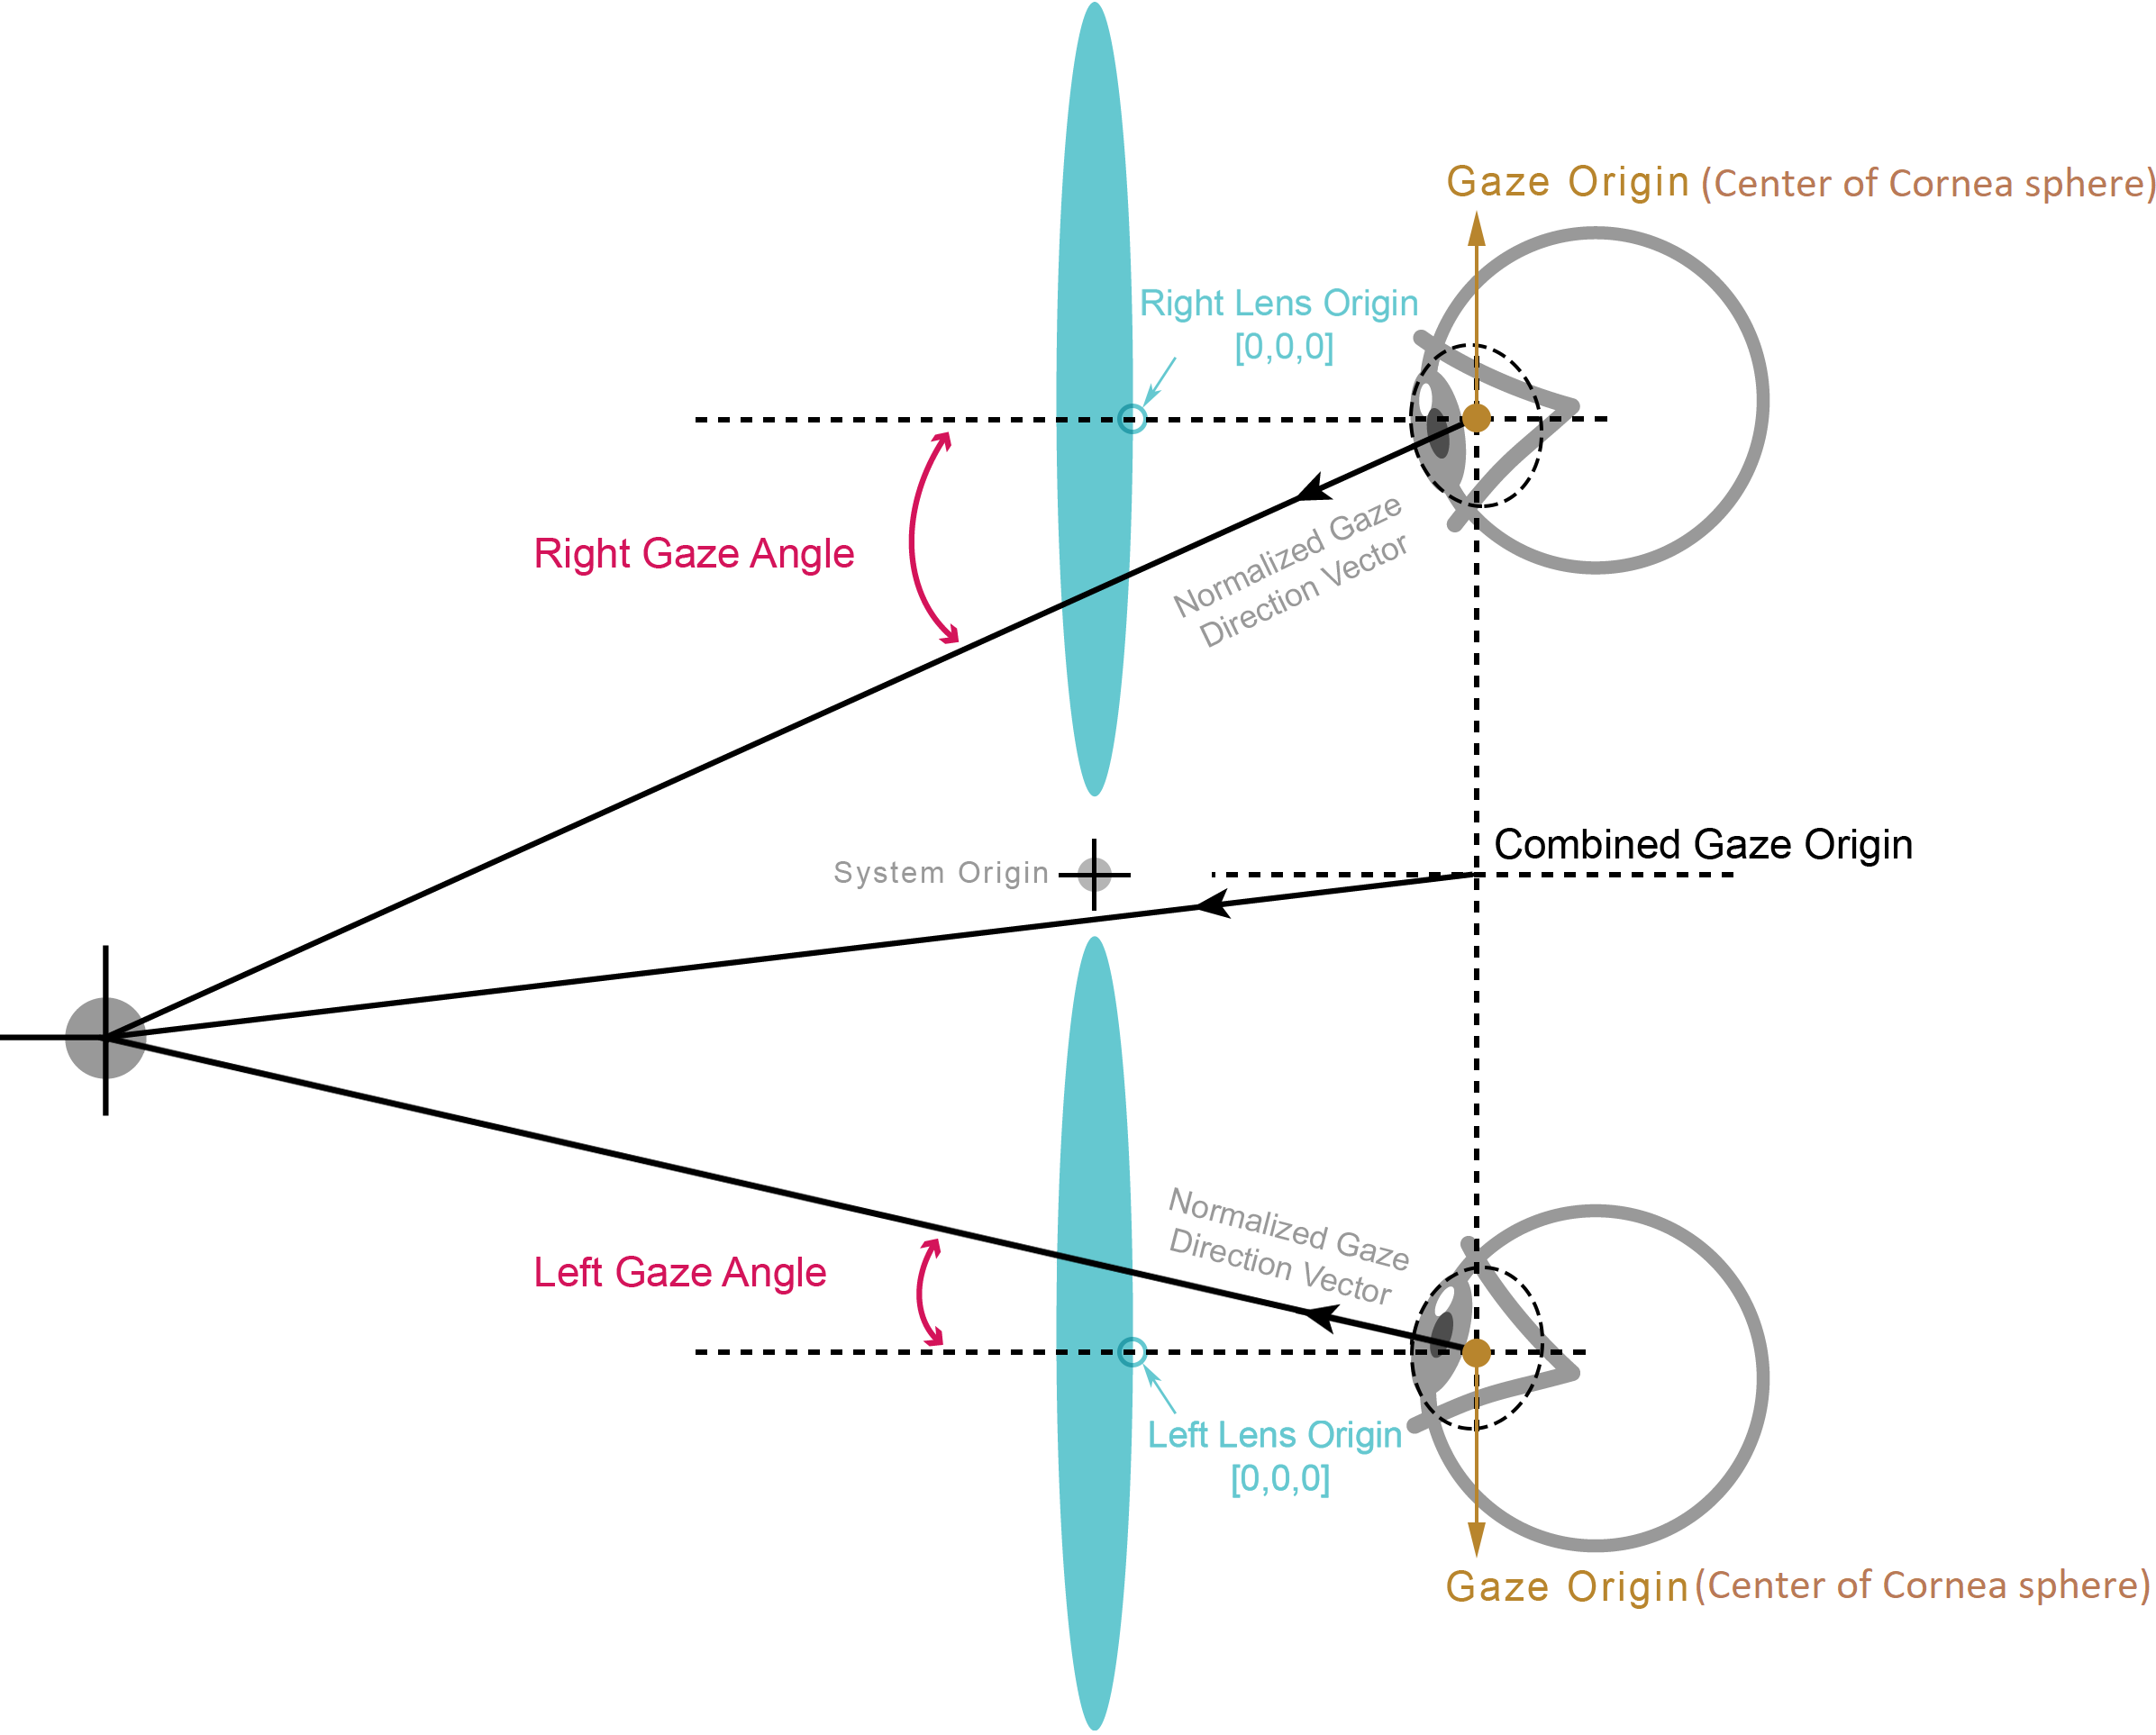
\includegraphics[width=\textwidth]{img/EyeData.png}
    \caption[Detailed scheme of gaze data]{Detailed scheme of gaze data~\cite{sranipal-image}}
    \label{fig:gaze-data}
\end{figure}

\pagebreak{}
\subsubsection*{Gaze structure}

Gaze data are the~result or output of an~ET device, but not every time the~data are suitable for the~use in a~virtual scene. Some eye trackers produce 2D coordinates on a~display surface that represent PoR~\cite{ugwitz2022}. If the~produced data are to~be used in a~virtual scene, it should be a~collection of 3D vectors. This is illustrated in Figure~\ref{fig:gaze-data}. The~gaze itself from a~single eye is represented by two 3D vectors;~normalised \emph{gaze direction} vector and \emph{gaze origin} coordinates.

Both are in a~coordinate system that is related to that particular eye. In this specific situation, the~origin of the~coordinate system is a~fixed point that is not related to the~eye itself because it can account for variations in the~eye positions of different people. Figure~\ref{fig:gaze-data} shows the~use of a~lens in HMD for VR as the~origin of the~eye's coordinate system.

\subsubsection*{Point of Fixation}
Subjects usually have two functioning eyes, so stereo gaze data can be used in their situation. Two separate coordinate systems, eye positions, and gaze directions. In the~best case, the~intersection of these two vectors in world coordinates can be used to~identify \emph{Point of Fixation} (PoF).

However, the~problem is that the~absolute precision of these vectors is not guaranteed due to~limitations in eye detection using video-based ET devices, which return acceptable results only for perfect calibrations. The~farther in a~scene the~eye gazes, the~more precision is required. In this case, the~accuracy must be below $0.5$ degrees.

The~difference between \emph{fixation} and PoF is that fixation describes the~type of gaze, and PoF is the~point in space where fixation occurs.

\subsubsection*{Combined gaze}
An~alternative to~stereo gaze data in multiple implementations of ET in HMDs is a~combined gaze vector. The~combined gaze origin is the~average of the~two origin coordinates, and the~direction of gaze is the~normalised sum of the~two gaze vectors. Each vector calculation is performed in the~ET device coordinate system.

\subsubsection*{Data processing}
To~search for fixations using the~combined gaze in the~scene, one has to~resort to~collisions. Sending a~ray in world coordinates from an~eye into the~scene -- \emph{raycasting}. PoF is the~first object (RoI) hit by the~ray.

The~search for fixations can be done in~real time during the~experiment or sometime after its end. In the~case of offline evaluation, it is first necessary to~gather the~scene information correctly together with the~gaze data during the~experiment. The~essential data consist of time in seconds or milliseconds, a~3D coordinate that reflects the~position of the~scene camera in the~world, its rotation, and the~gaze origin with its direction; two 3D vectors in world coordinates.

These are saved in a~CSV file or in an~internal database. During prototype testing, it is more convenient to~save data in CSV because the~file can be deleted at any time after a~failure, as opposed to~deleting non-valid entries from a~database. Performing offline computations is meaningful only when the~gaze data are processed and visualised in several different ways that clearly consume computational power. If a~search for PoF is performed alone, there is no reason not to~compute it in real time.

\pagebreak{}
\subsection{Visualisations}

Analysing the~existing solutions later in Section~\ref{sec:solutions} found that there are generally two ways to visualise gaze data in a~virtual environment. Many analyses of gaze data consist of recording them in external files and processing or visualising them with a~help of a~statistical programme. The~basis for all visualisations are PoFs in 3D space. These points are then transformed or classified into more specific structures. 

\begin{description}
    \item[Heatmap] is a~graphical representation of data where each value on a~map is represented by a~colour from a~predetermined spectrum. Typically, this is a~transition from blue, representing the~minimum value, through green and yellow to red, which indicates the~maximum value. In the~context of fixations, higher heatmap values are indicative of a~denser concentration of PoFs or their individual strength; the~duration of fixation.
    \item[Gaze trail] is a~visual representation of \emph{scanpath}, where PoFs are displayed by a~simple cube or sphere primitive. Saccades connect these primitives in space with lines.
\end{description}

This interesting study from 2005 explores attention search in a~virtual environment~\cite{kit2014}. This is an~experiment that explores visual search for different objects in a~virtual three-room apartment with the~participation of several subjects over multiple days.
They used a~custom HMD with lower resolution to~collect the~data, given the~age of the~study. Eye images, camera view, and participant's position in the~scene were recorded for an~evaluation. The~whole situation was reconstructed offline for analysis.

The~PoF was obtained using an~algorithm that took the~eye position from an~eye image and used its screen coordinates to~extract a~60x60 pixel square from the~camera scene footage. From these few pixels, it was evaluated which object occupied the~most pixels. The~same object's location was used as the~3D fixation coordinate.

It is possible to~visualise 3D data by condensing them onto a~2D map. They created several graphs and 2D heatmaps from the~gathered PoFs. For example, the~floor plan of an~experiment scene can be overlaid with a~heatmap that describes the~spatial intensity of gaze data.

\begin{figure}[!ht]\centering
    \begin{subfigure}[b]{0.4\textwidth}
        \centering
        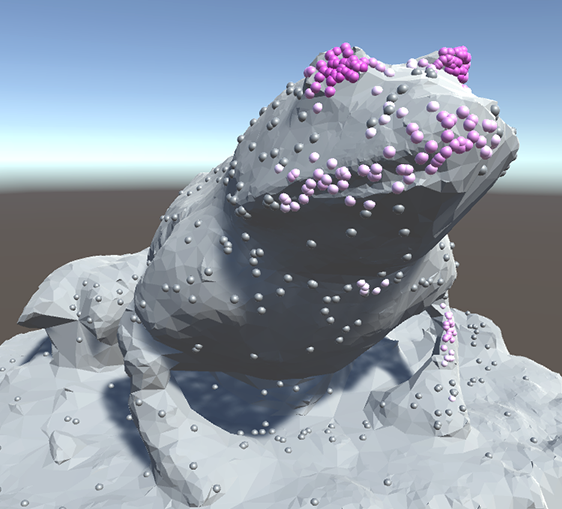
\includegraphics[width=0.9\textwidth]{img/ugwitz-heatmap.png}
        \caption{3D Heatmap points~\cite[p. 52]{ugwitz2020thesis}}
        \label{fig:ugwitz-heatmap}
    \end{subfigure}
    \hfill
    \begin{subfigure}[b]{0.55\textwidth}
        \centering
        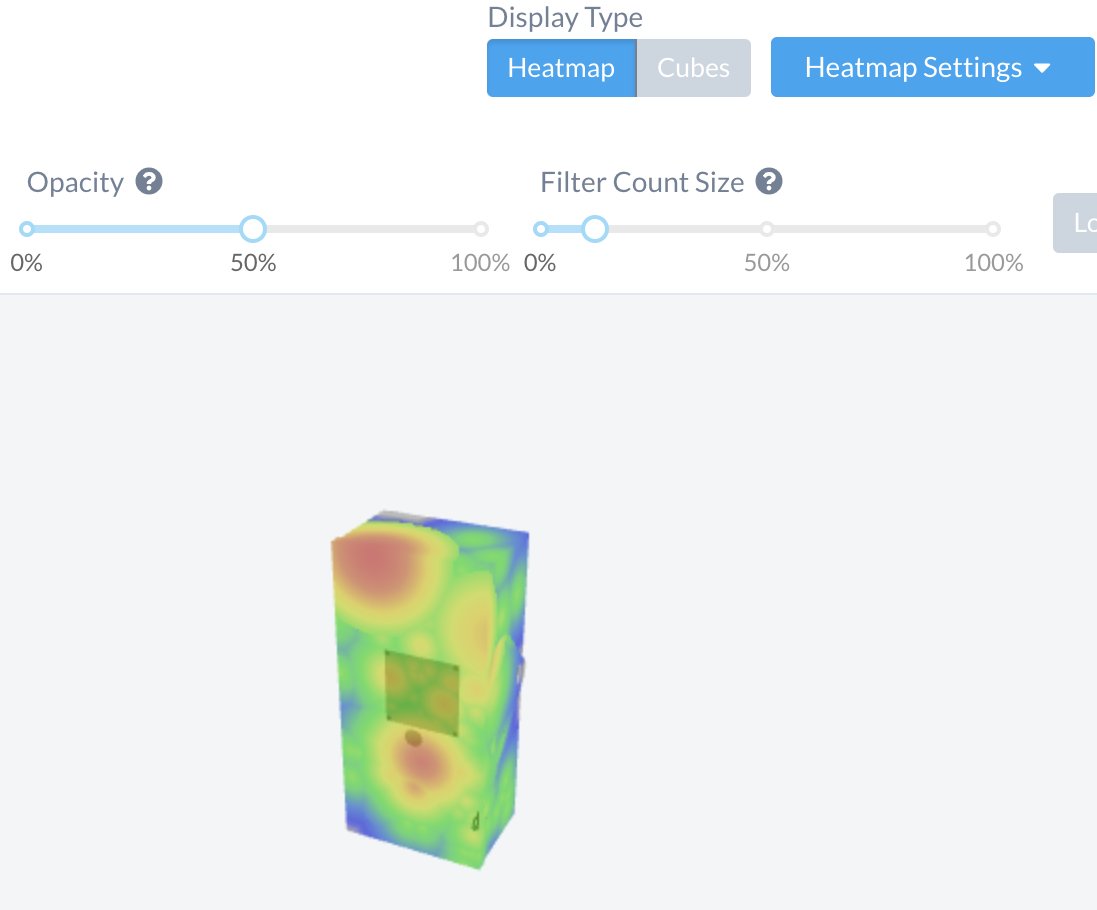
\includegraphics[width=\textwidth]{img/cognitive3d-heatmap.png}
        \caption{Object texture heatmap~\cite{cognitive3d-dynamic-objects}}
        \label{fig:cognitive-heatmap}
    \end{subfigure}
    \caption{Example of two different heatmap approaches.}
\end{figure}

\pagebreak{}
This paper~\cite{ugwitz2022}, which is closely related to a~thesis by the~same author~\cite{ugwitz2020thesis}, visualises heatmaps using 3D points in space that are coloured differently according to the~intensity of a~given fixation, can be seen in Figure~\ref{fig:ugwitz-heatmap}.

Cognitive3D software visualises gaze data using heatmaps and visual trail. Heatmaps are generated in a~different way. They draw it on the~wireframe of a~3D model -- Figure~\ref{fig:cognitive-heatmap} -- assumably onto a~texture. The~algorithm they use to do this is proprietary. For real-time visualisation of gaze data, without the~need to collect and evaluate the~data offline, the~method of drawing heatmaps on objects is more suitable. 


\section{Current hardware}
\label{sec:hardware}

ET devices implemented in VR HMDs are portable devices that have only recently seen their first prototypes. The~same applies to the~first truly usable VR headsets that have started to~appear since Oculus' first attempt with its \emph{Rift DK-1} headset. This was immediately followed by the~\emph{DK-2} version. HTC joined in on~this with their VIVE headset. They were all released in a~short period of time before 2016, which is exactly the~year when all the~aforementioned were extended with an~SMI eye tracker.~\cite{ugwitz2022}

Unfortunately, SMI announced that it discontinued the~production and support of its ET devices when it was acquired by Apple in 2017~\cite{iMotions-endSMI}. Regardless of this whole situation, Tobii created an~ET Development Kit for HTC VIVE that was not bundled with the~heatset itself. It had to be purchased separately and mounted inside a~very confined space around the~lenses~\cite{tobii-oldHTC}. Modern headsets are made with ET integrated into them by design. Manufacturers have two options. They either develop ET devices themselves as their proprietary solution or leave it to a~third-party. One of them is Tobii, which dominates the~ET market.~\cite{ugwitz2020thesis}

\subsection{Tobii}
This company is exclusively specialised in eye tracking. Since their inception, when they released the~world's first plug-and-play ET device in 2002~\cite{tobii-history}, they have grown to~become a~global leader in the~industry.

\subsubsection*{Design}
Current Tobii eye tracking systems are based on non-intrusive video-based tracking that uses the~PCCR method. Their implementation uses multiple NIR light sources to~create reflexion patterns, several glints, on the~cornea and pupil, which are recorded by cameras. They use an~advanced image processing algorithm based on a~physiological 3D eye model to~detect the~eye and estimate the~gaze.~\cite{tobii-eye-trackers}

Most of their devices use the~dark and bright pupil method for eye detection, except for wearable devices that use only the~dark pupil method. All~of their devices use the~method mentioned using a~3D eye model for gaze estimation.~\cite{tobii-dark-pupil}

\subsubsection*{Wearable device}
An~example of their wearable eye trackers is Tobii Glasses 3, shown in Figure~\ref{fig:tobii-glasses3}. The~device is designed to~handle real-world ET research. A~robust system is in place, consisting of eight NIR illuminators for each eye separately that create glints. The~single eye with glints is then captured by two very small cameras with a~sampling rate of 100 Hz. A~one-point calibration is performed before measurement. The~device is also equipped with a~full HD camera, which is located in the~beam of glasses. It is a~portable device that does not require a~connection to a~PC, as the~product includes a~recording unit that captures video from the~camera and simultaneously collects ET data to an~SD card. The~accuracy of the~measured data is around $0.6^{\circ}$. The~data are processed and visualised using their analytics software, Tobii Pro Lab. Their Tobii Pro Glasses 3 API allows for a~custom implementation.~\cite{tobii-glasses3}

\begin{figure}\centering
    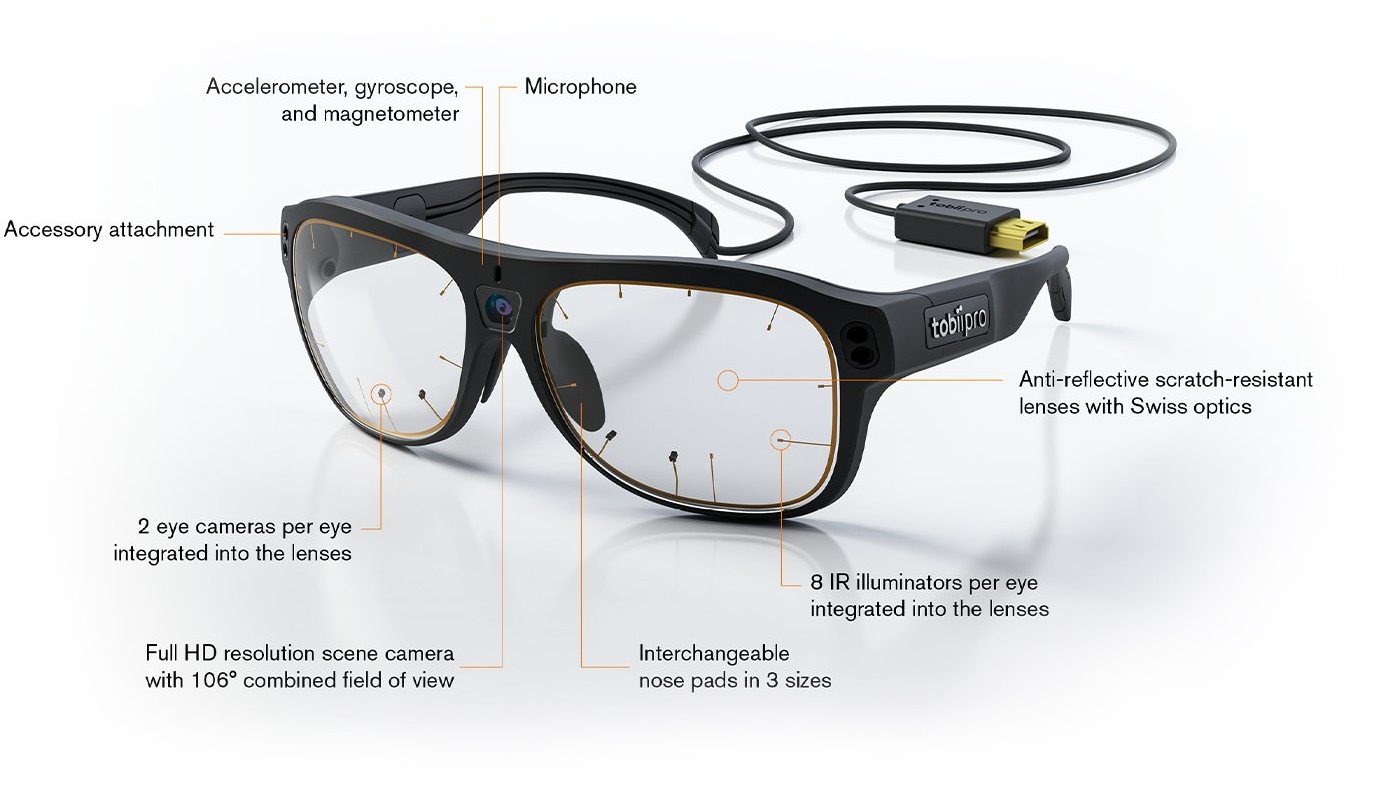
\includegraphics[width=0.9\textwidth]{img/TobiiGlasses3.jpg}
    \caption[Description of Tobii Glasses 3.]{Description of Tobii Glasses~3.~\cite{tobii-glasses3-image}}
    \label{fig:tobii-glasses3}
\end{figure}

\subsubsection*{Table-mounted device}
Tobii also develops table-mounted devices, one of which is the~Tobii Pro Fusion. It is an~ET device that consists of two cameras with a~sampling rate of 250 Hz. The~dual camera setup is used for better head movement tolerance. The~accuracy of this device is $0.3^{\circ}$. Gaze data can be collected and used in their proprietary Tobii Pro Lab software or with the~Tobii Pro SDK, that allows for integration in C, Python programming language,.NET framework or \emph{Unity} game engine.~\cite{tobii-fusion, tobii-pro-sdk}

\begin{figure}[!b]\centering
    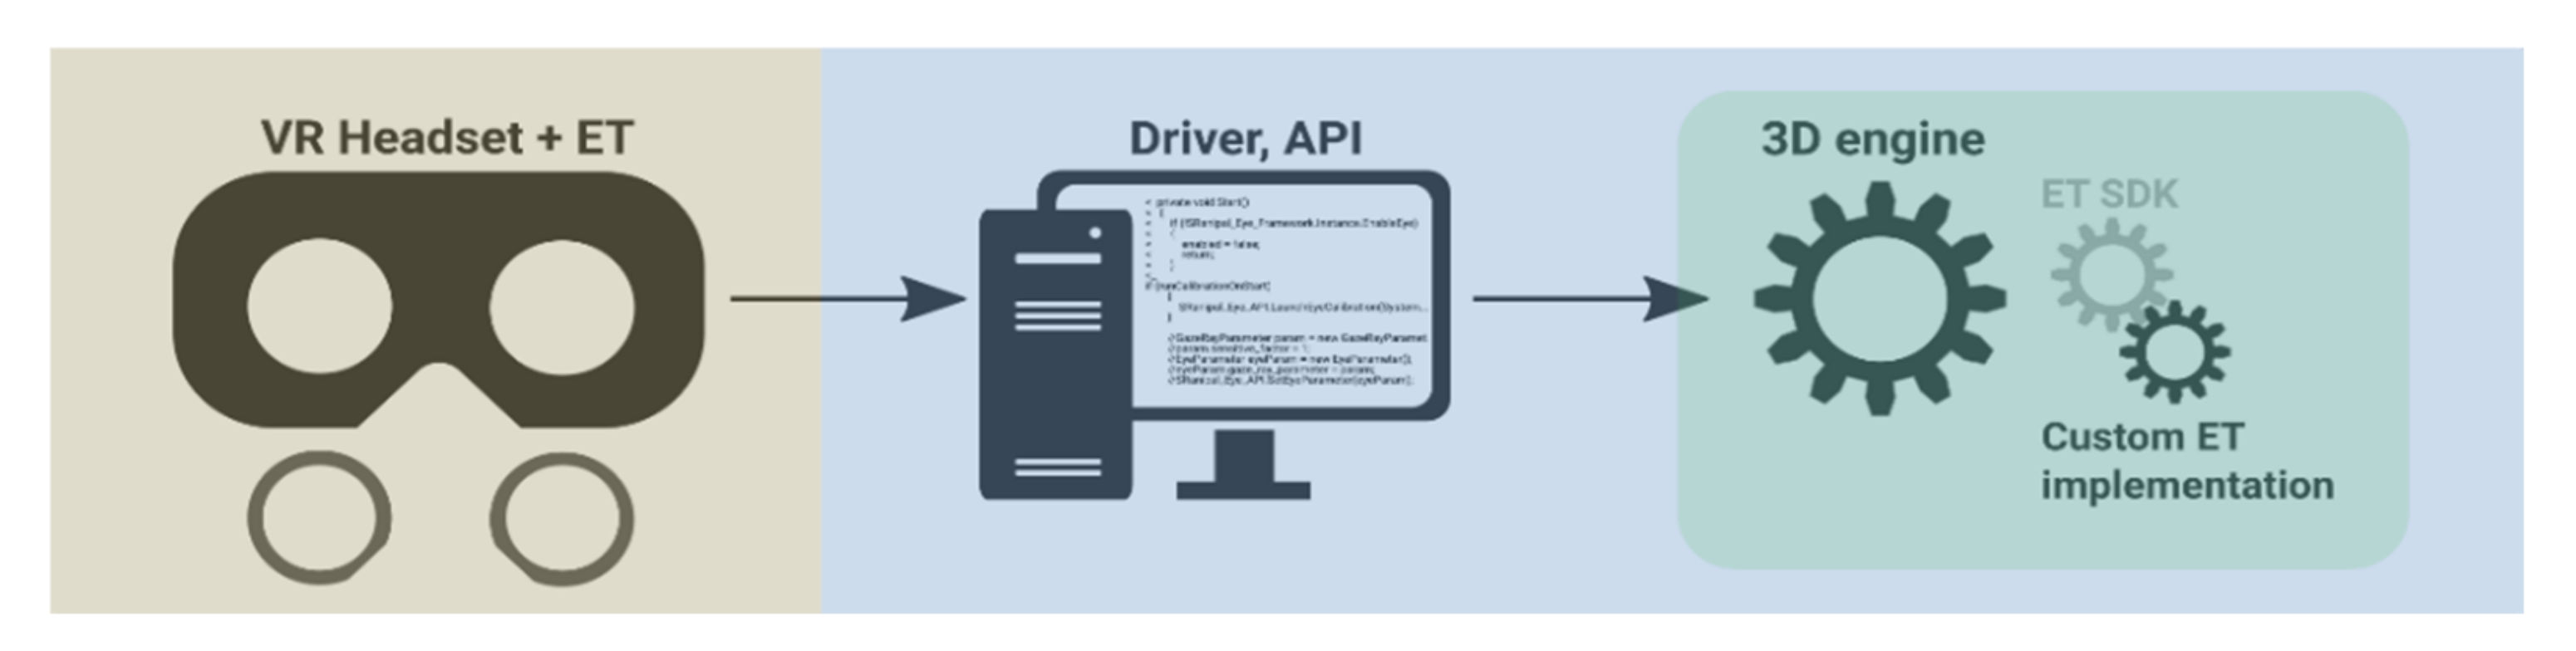
\includegraphics[width=\textwidth]{img/ET-SDK.jpg}
    \caption[Interconnection of ET hardware with SDK.]{Interconnection of ET hardware with SDK.~\cite[p.~4]{ugwitz2022}}
    \label{fig:et-sdk}
\end{figure}

\newpage

\subsection{Integrations in VR HMDs}
\label{sec:integrations}

In~addition to Tobii's own eye trackers, the~company has partnered with various VR headset manufacturers to~provide integration of their ET units. These are HTC, PICO, and HP. Specifically, the~headsets with integrated ET from Tobii include HTC VIVE Pro Eye, HP Reverb G2 Omnicept Edition, PICO Neo 2 Eye and Neo 3 Pro Eye. A~comparison of these devices can be found in Table~\ref{tab:headset-tech-tobii}, which shows their specifications. Frequency of the~output gaze data, measurement accuracy, calibration method, trackable \emph{field of view} (FOV), available \emph{Software Development Kit} (SDK), type of output gaze data, the~state of OpenXR standard implementation, and SDK support for the~two major game engines.

\renewcommand{\arraystretch}{1.15}
\begin{table}[!ht]
\centering
\begin{tabular}{|l||c|c|c|}
\hline
\multicolumn{1}{|c||}{} &
  \begin{tabular}[c]{@{}c@{}}HTC VIVE\\ Pro Eye \cite{tobii-htc-vive}\end{tabular} &
  \begin{tabular}[c]{@{}c@{}}HP Reverb G2\\ Omnicept Edition \cite{tobii-hp-omnicept}\end{tabular} &
  \begin{tabular}[c]{@{}c@{}}PICO Neo 3\\ Pro Eye \cite{tobii-pico3}\end{tabular} \\ \hline\hline
Frequency     & 120 Hz       & 120 Hz          & 60/90 Hz          \\ \hline
Accuracy      & $0.5^{\circ}$--$1.1^{\circ}$    & $<1.0^{\circ}$  & $<1.0^{\circ}$ \\ \hline
Calibration   & 5-point      & 9-point         & 5-point        \\ \hline
Trackable FOV & $110^{\circ}$ & $114^{\circ}$  & $101^{\circ}$  \\ \hline
SDK           & HTC SRanipal & HP Omnicept SDK & Pico SDK       \\ \hline
Stereo gaze    & Yes & Yes    & No     \\ \hline
Combined gaze    & Yes & Yes    & Yes     \\ \hline
%OpenXR Ready  & Yes           & Yes             & Yes            \\ \hline
OpenXR  & Yes           & Yes             & Ready            \\ \hline
Unreal, Unity & Both & Both & Both \\ \hline
\end{tabular}
\caption{Specification of the~latest VR headsets with Tobii ET integration.}
\label{tab:headset-tech-tobii}
\end{table}

\subsubsection*{Software Development Kit}
HMDs communicate with software using a~driver. SDKs are used to add the~communication functionality to the~software. This set of development tools is provided by the~hardware manufacturer. In the~case of VR implementations, the~SDK is in the~form of an~\emph{Application Programming Interface} (API) that returns the~requested data to the~application from some VR runtime that is part of the~hardware driver. As~Figure~\ref{fig:et-sdk} illustrates. 

\subsubsection*{Tobii SDK}
One SDK is available for all HMDs with a~Tobii eye tracker; Tobii XR SDK. The~strength of using this is the~unified access to the~data across all devices. On the~other hand, it offers a~stable release only for the~\emph{Unity} game engine. \emph{Unreal Engine} SDK is still in beta version\footnote{does not work with HTC VIVE Pro Eye} and support for native~C development is only in Alpha. In contrast to~all the~dedicated device SDKs listed in Table 2.1, which offer full support for the~mentioned game engines and native~C.~\cite{tobii-xrsdk} 

\pagebreak{}

\subsection{OpenXR standard}
Until recently, for an~application to be able to use a~specific VR device, a~proprietary API was required to communicate with its hardware driver. Support for different devices in one app required custom driver integration. However, the~Khronos Group has proposed a~new standard to fight this fragmentation; \emph{OpenXR}, which provides high performance cross-platform access to~\emph{Augmented Reality} (AR), \emph{Mixed Reality} (XR) and \emph{Virtual Reality} devices and platforms. 

This includes not only HMDs, but also VR controllers, hand tracking, and eye tracking. New applications are now able to~share the~same interface to~communicate with several different VR, XR, or AR devices, as the~schema on Figure~\ref{fig:openxr-schema} shows. OpenXR is not a~library or an~implemented runtime, but a~specification of how that runtime should look. The~implementation is done by XR device manufacturers themselves.~\cite{openxr-overview, openxr-presentation}

\begin{figure}[!ht]\centering
    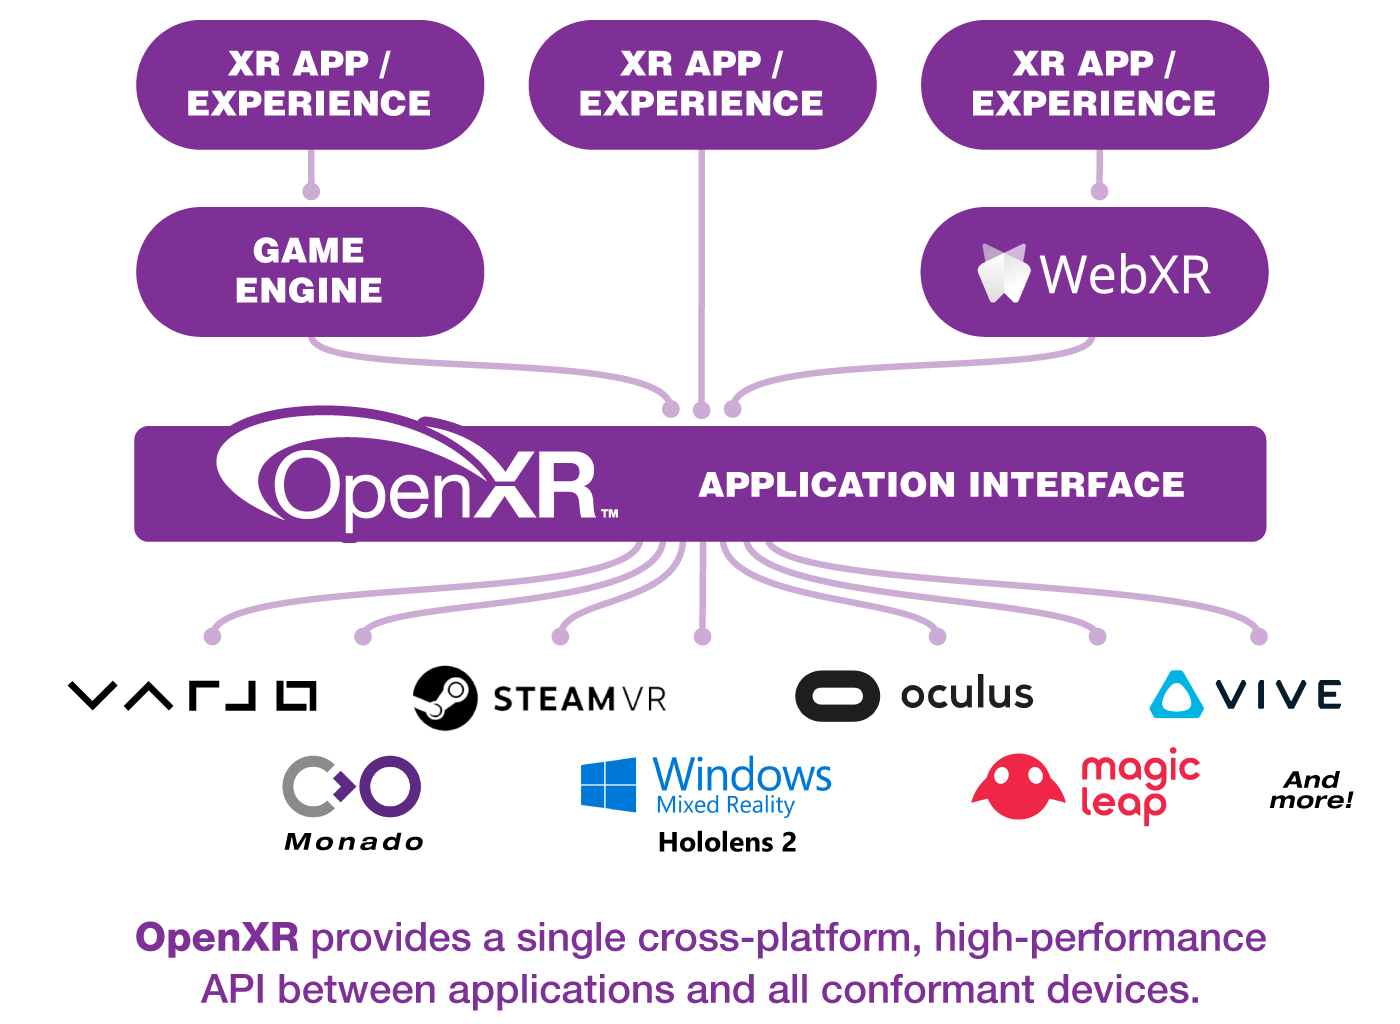
\includegraphics[width=0.75\textwidth]{img/openXR.png}
    \caption[Schema of OpenXR cross-platform access to different XR devices.]{Schema of OpenXR cross-platform access to different XR devices.~\cite{openxr-access-image}}
    \label{fig:openxr-schema}
\end{figure}

An~important aspect of OpenXR is that it uses a~Cartesian right-handed coordinate system to describe the~space in which all vectors are represented; the~$x$ coordinate points to the~right, the~$y$ points up, and the~$z$ coordinate points backward ($-z$ points forward into the~scene).~\cite{openxr-coordinate}

\subsection{Varjo}
\label{sec:varjo}

Varjo is a~Finnish manufacturer of VR and XR HMDs. Their latest VR devices are VR-3 (Figure \ref{fig:varjo-vr3}) and the~Aero headset. All Varjo devices are equipped with Varjo's own proprietary ET solution, not based on Tobii. They claim that their method is ``the~most accurate eye tracking ever integrated into a~VR device''.~\cite{varjo-et}

\subsubsection*{Method}
It is a~method based on 2D regression that is enhanced by the~type of illuminators and camera quality. It uses a~special custom IR illuminator shape that produces complex-shaped glints, instead of dots.

The~robustness of this solution lies in the~ability to~use computer vision algorithms to~distinguish one illuminator from another by examining the~orientation of its glint. Combined with IR cameras that capture eye images at 100~\emph{frames per second} (fps) at a~resolution of 1280x800 pixels, the~accuracy of eye measurement is guaranteed to~be sub-zero degrees even when the~eyes are looking at extreme angles or when glasses are present.

\subsubsection*{Capabilities}
Both headsets are capable of producing combined and stereo gaze output data at 200~Hz. They include an~automatic PID (auto-PID) capability to~adjust the~lens distance and foveated rendering after a~single-point calibration. What~VR-3 has over the~newer and lighter Aero is a~built-in Ultraleap camera for hand tracking, which is visible in Figure~\ref{fig:varjo-vr3}. Headsets use the~native Varjo SDK or OpenXR runtime~\cite{varjo-openxr} to~communicate with apps. Offers support for implementation in native~C and integration into Unreal Engine and Unity game engine.~\cite{varjo-vr3, varjo-aero}

Gaze data output is natively in the~left-handed coordinate system. The~vectors are then represented in a~space where $x$ points to the~right, $y$ points up and $z$ points forward in the~scene; compared to OpenXR, the~z coordinate is flipped. To~start ET, the~device must first be calibrated. This can be done in three different ways. Either a~five-point calibration, which uses statistical data collected from previous calibrations by other users to~enhance the~calibration result, or a~ten-point legacy calibration, which does not include such a~feature. One point cannot be used to~initiate ET, it only serves to~activate foveated rendering.~\cite{varjo-sdk-spec}

\begin{figure}[!t]\centering
    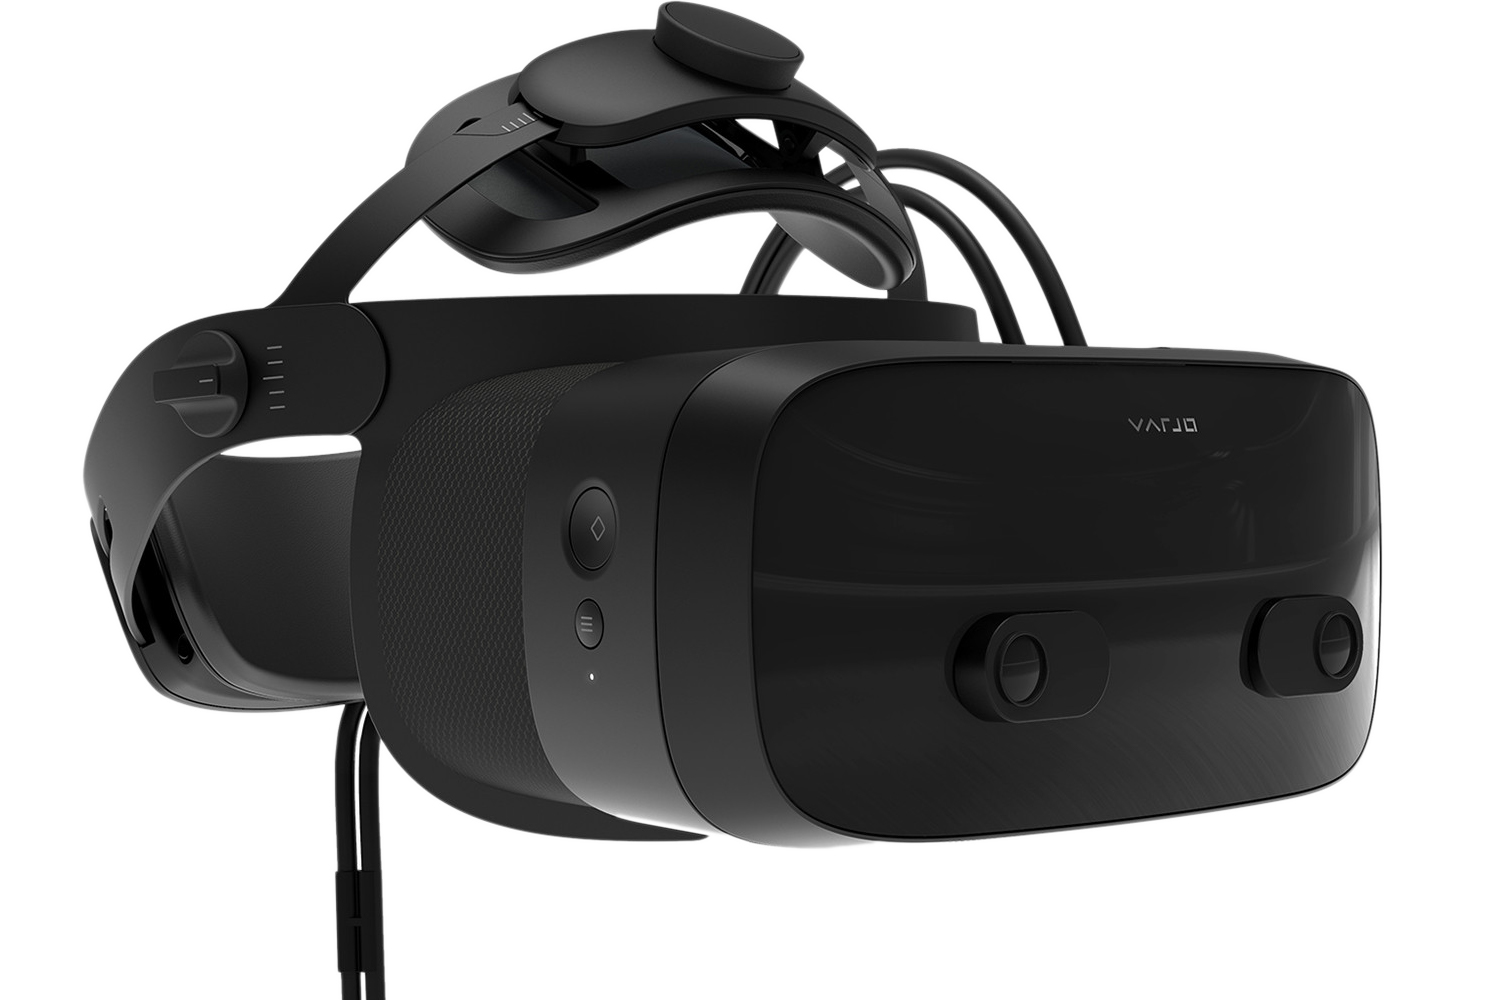
\includegraphics[width=0.7\textwidth]{img/Varjo-VR3.jpg}
    \caption[Varjo VR-3 virtual veality headset.]{Varjo VR-3 virtual reality headset.~\cite{varjo-vr3-image}}
    \label{fig:varjo-vr3}
\end{figure}

Varjo driver has built-in tools to~record gaze data. This feature records them simultaneously with a~video of what the~user has seen. The~output is a~.csv file that can be used to~visualise the~data collected in the~recorded video. The~CSV contains generic gaze data along with their transformation into video coordinates. The~generic data contain the~origin and direction of the~gazes of the~left and right eye and their combined gaze with a~raw timestamp of when the~data were recorded. The~second data in relation to the~video are transformed into 2D coordinates (PoR) and stored together with the~timestamp relative to the~start of the~video.~\cite{varjo-data-logging}


\subsubsection*{Immersive Virtual Reality}
Another Varjo device is the~XR-3 headset for mixed reality, which is almost identical to the~VR-3 but includes the~feature of a~video feed of the~external world. This headset uses two cameras to~record video that can be modified and rendered back on the~internal displays.~\cite{varjo-xr3}

\emph{Immersive Virtual Reality} (IVR) is a~3D projection used in Religious Studies testing Laboratory build by Olomouc Palacký University.~\cite{upol2021procurement}

\begin{figure}[!ht]\centering
    \begin{subfigure}[b]{0.38\textwidth}
        \centering
        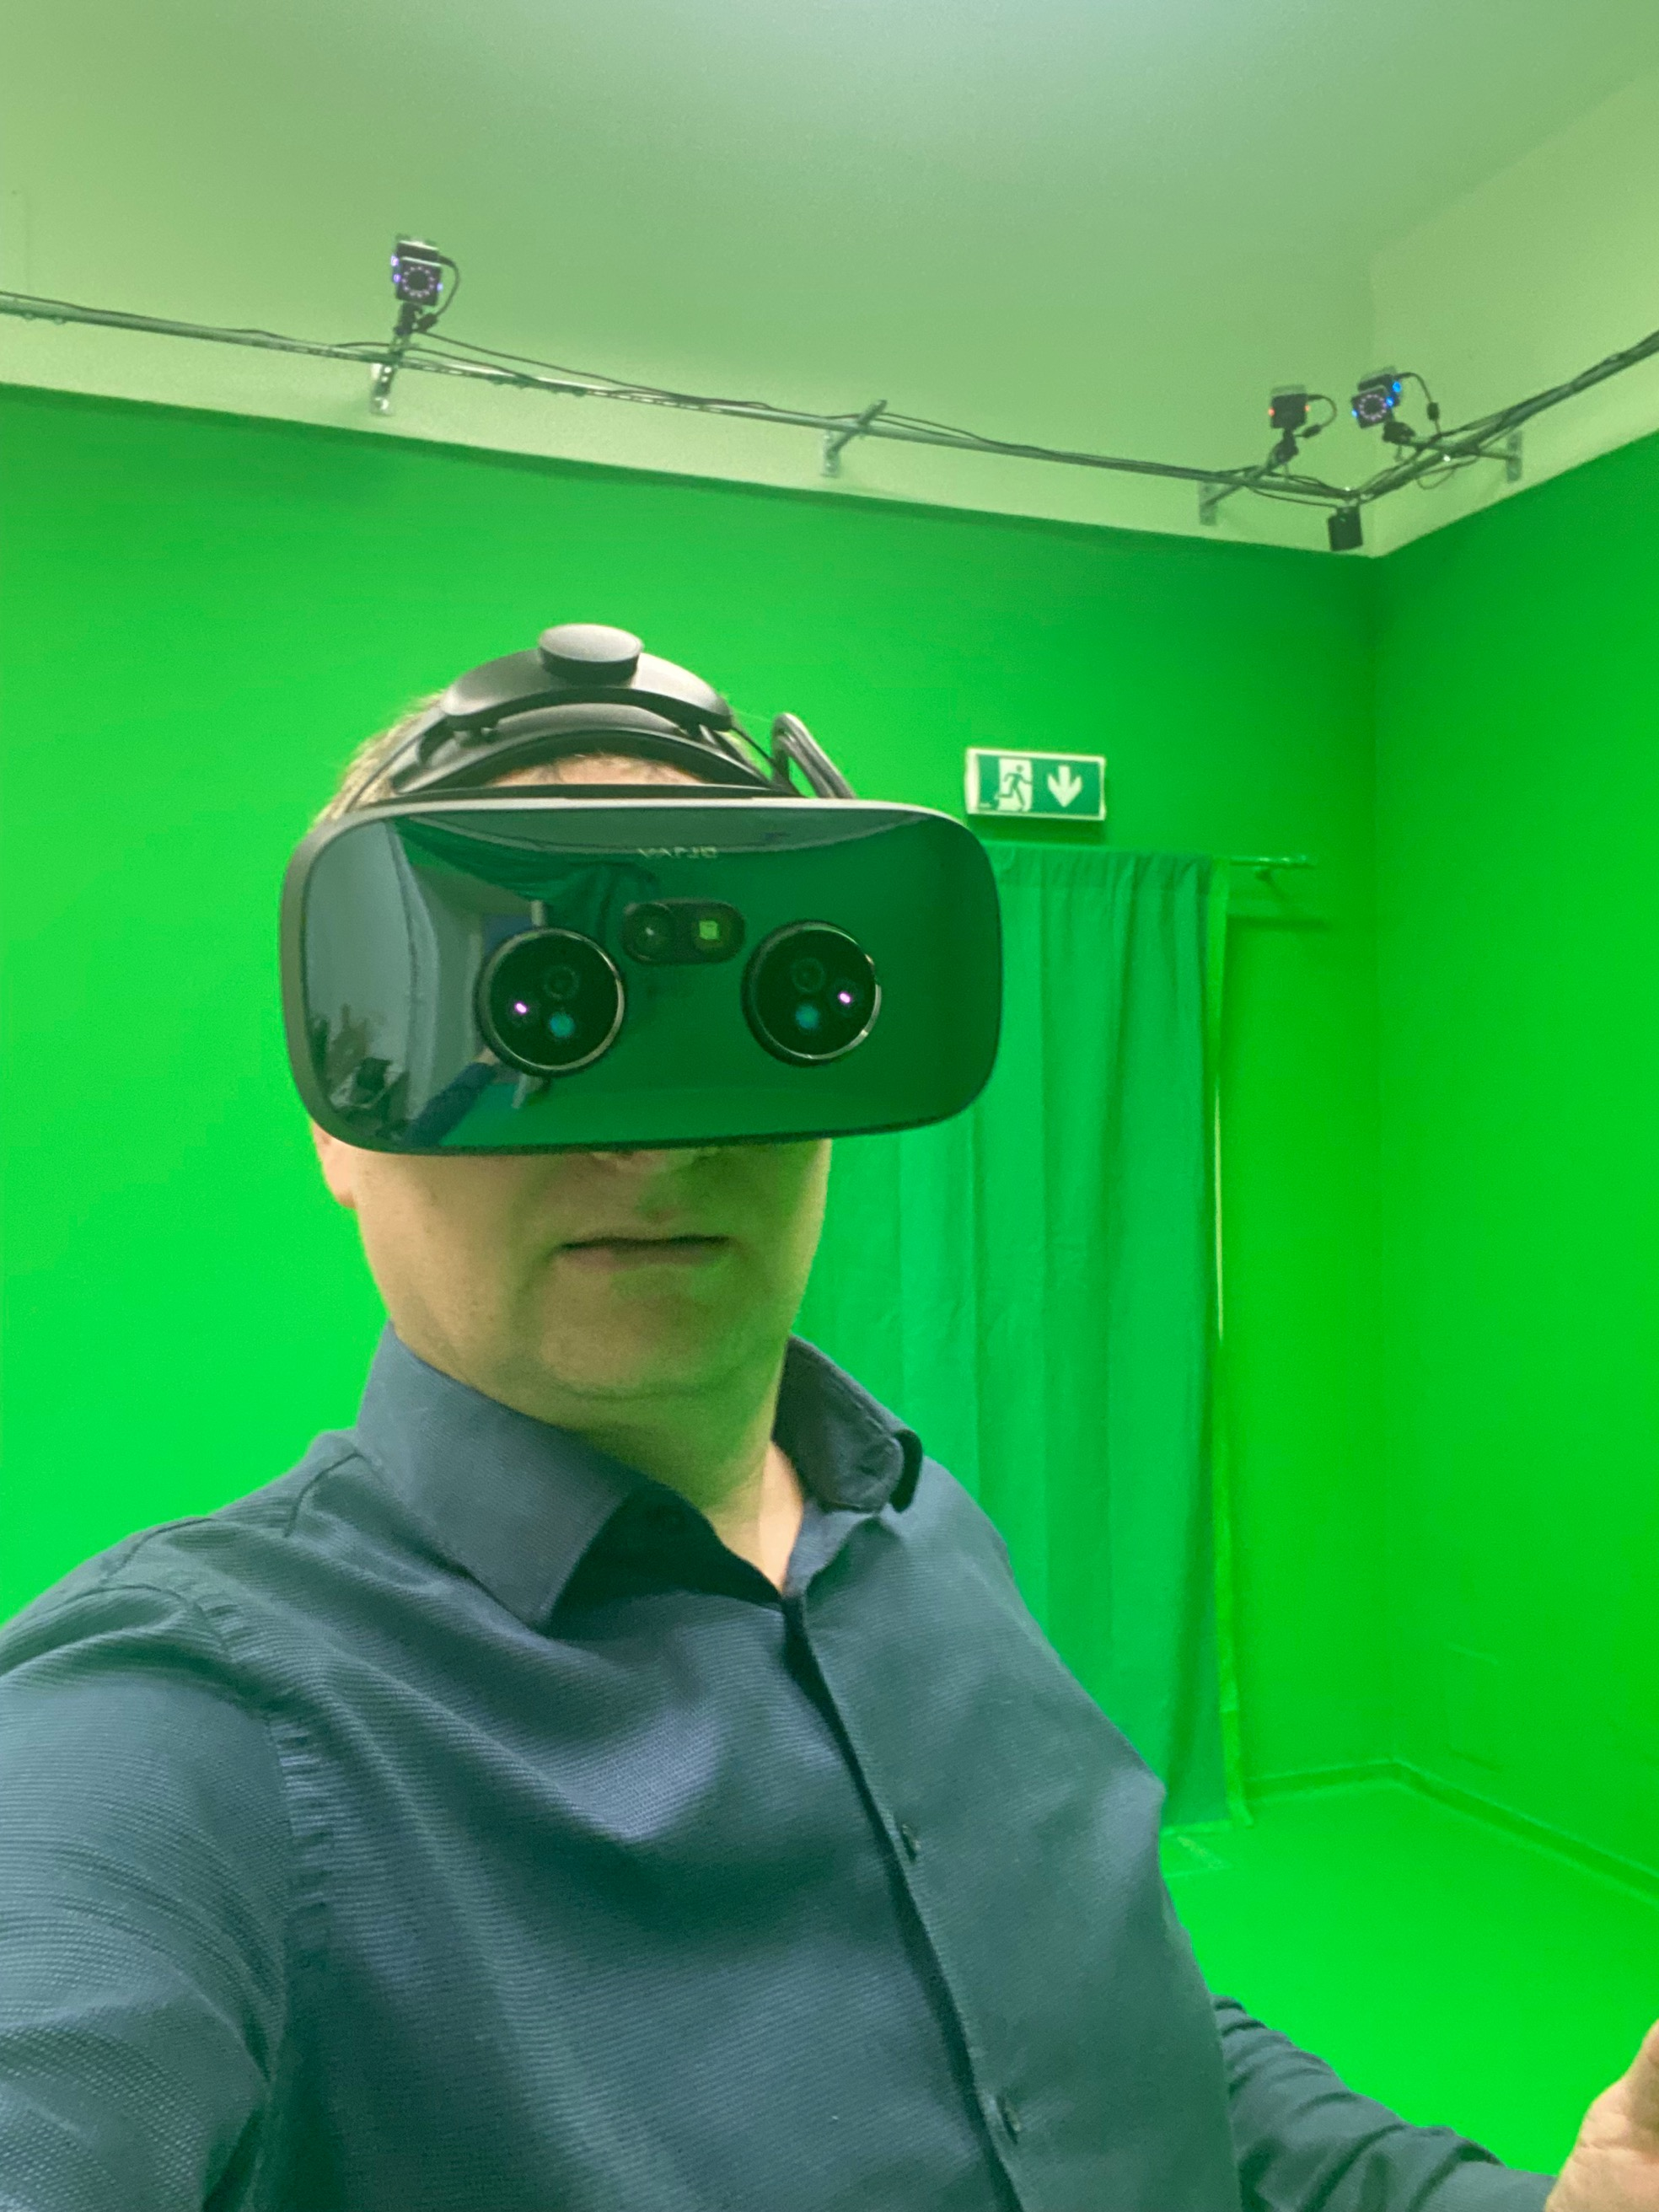
\includegraphics[width=0.89\textwidth]{img/ivr-supervisor.png}
        \caption{Varjo XR-3 headset in use.}
        \label{fig:ivr-sup}
    \end{subfigure}
    \hfill
    \begin{subfigure}[b]{0.6\textwidth}
        \centering
        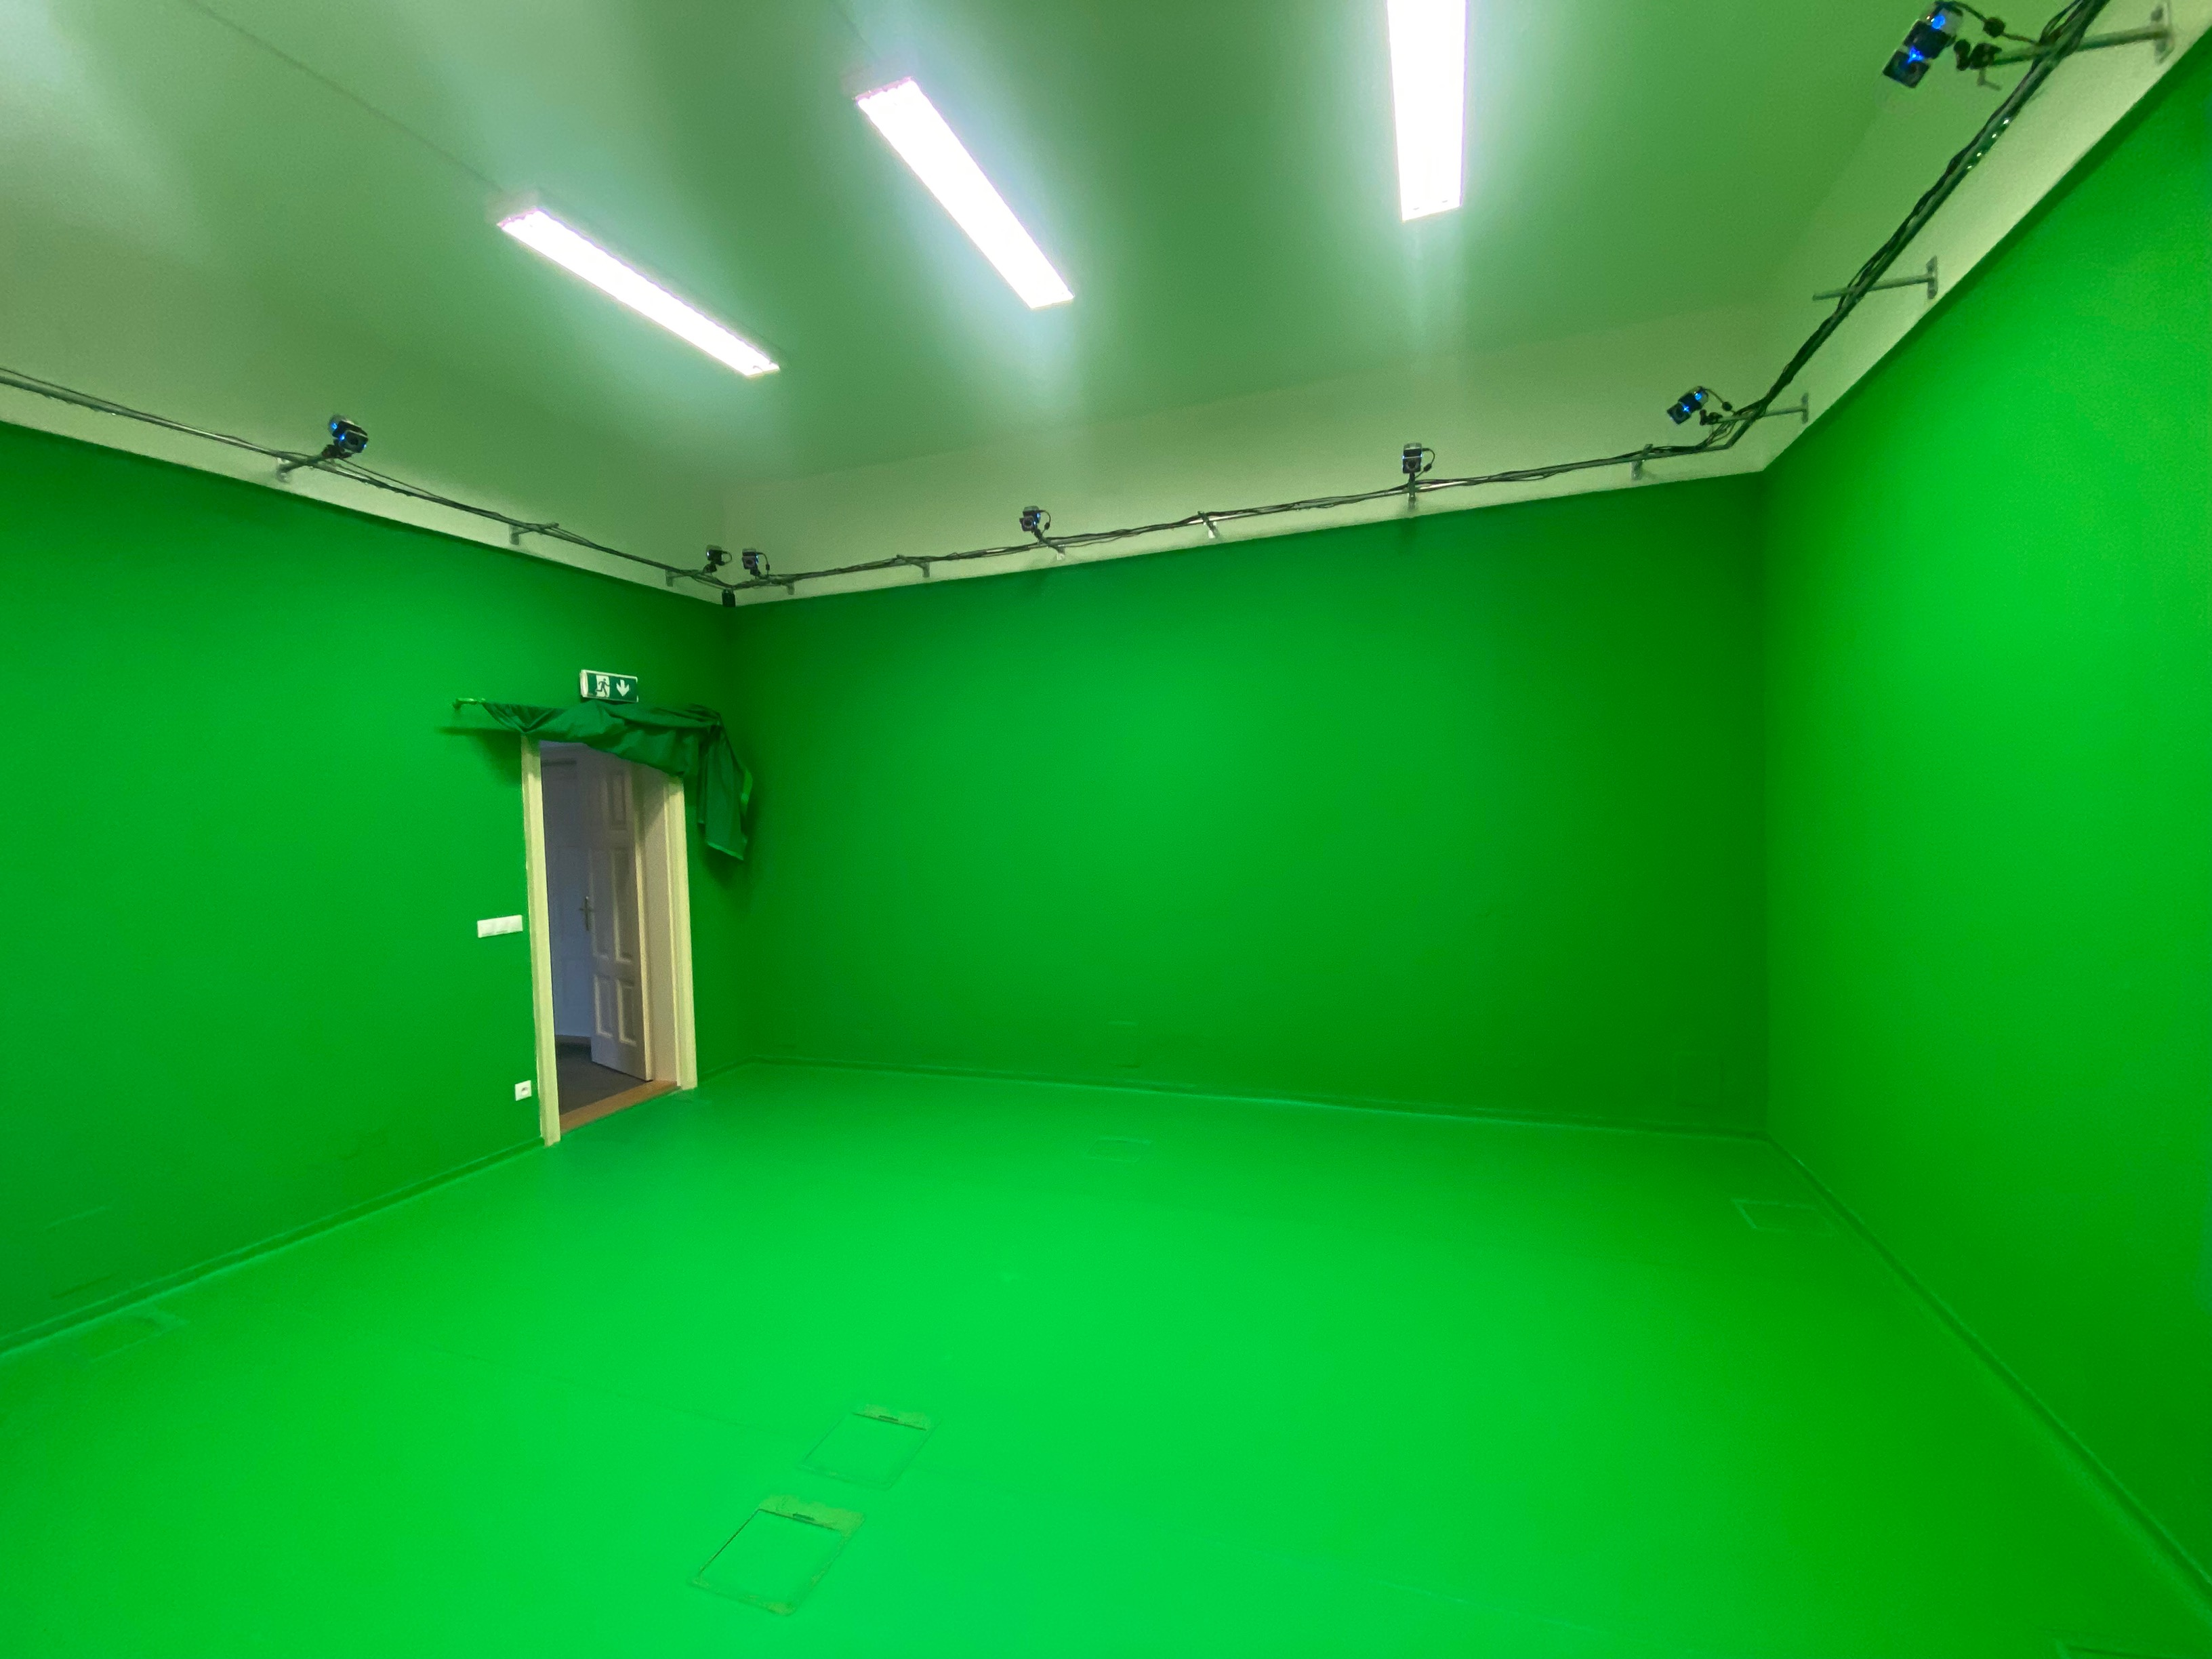
\includegraphics[width=\textwidth]{img/ivr-lab.png}
        \caption{Interiour of the~laboratory.}
        \label{fig:ivr-lab}
    \end{subfigure}
    \caption{Mixed reality laboratory for religious studies in Olomouc Palacký University.}
\end{figure}

This Czech lab uses the~aforementioned XR headset and its ET capabilities to~record and study human behaviour during religious processes. The~headset records a~video of the~lab, and then the~green screen is keyed out during the~post-process. The~result is used to~overlay the~virtual scene that is displayed later inside the~headset. They use VICON's tracking system to~track the~position of the~headset. The~system uses a~multiple camera setup, some of which can be seen in Figure~\ref{fig:ivr-lab}.

\subsection{Vrgineers XTAL}
\label{sec:xtal}

Vrgineers is a~Czech-American company that has been making VR headsets since 2016. Their hardware is called XTAL, and all of its versions include built-in ET hardware. The~latest XTAL is in version 3~\cite{vrginners-xtal3-spec}, Figure \ref{fig:vrg-xtal3}, which also exists in a~version for XR that includes additional cameras that project the~outside world inside. 

\subsubsection*{Features}
Headsets consists of several features. They offer auto-IPD, hand tracking with the~help of Ultraleap cameras, and an~ET system that consists of two arrays of several IR light dots, one for each eye, to~which a~single IR camera is paired. An~IR camera has a~resolution of 1280x800 pixels, which is captured at 110~Hz frequency. ET operates natively at 120~Hz, but it is possible to~increase the~frequency of the~eye tracker's output data up to 210~Hz.~\cite{vrginners-xtal-spec}

\subsubsection*{Runtime}
At the~time of writing, the~XTAL headsets communicated only using their stable native VRG runtime, which uses this ET system only for IPD measurement and foveated rendering. This was not entirely clear at the~beginning of the~investigation and was believed to be capable of returning gaze data because the~source code of their SDK included gaze data structures similar to those presented in Section~\ref{sec:gaze-data}. However, Vrgineers support later informed that they were developing another runtime that was capable of this.

Their~goal is to~convert the~entire native runtime to~OpenXR, which is currently in beta and already offers left, right, and combined gaze data according to the~OpenXR specification. The~native runtime offer support for native C development and integration to Unreal and Unity. They tested the~beta OpenXR runtime on Unreal Engine versions 4.27 and 5.~\cite{vrginners-email}

\begin{figure}[!t]\centering
    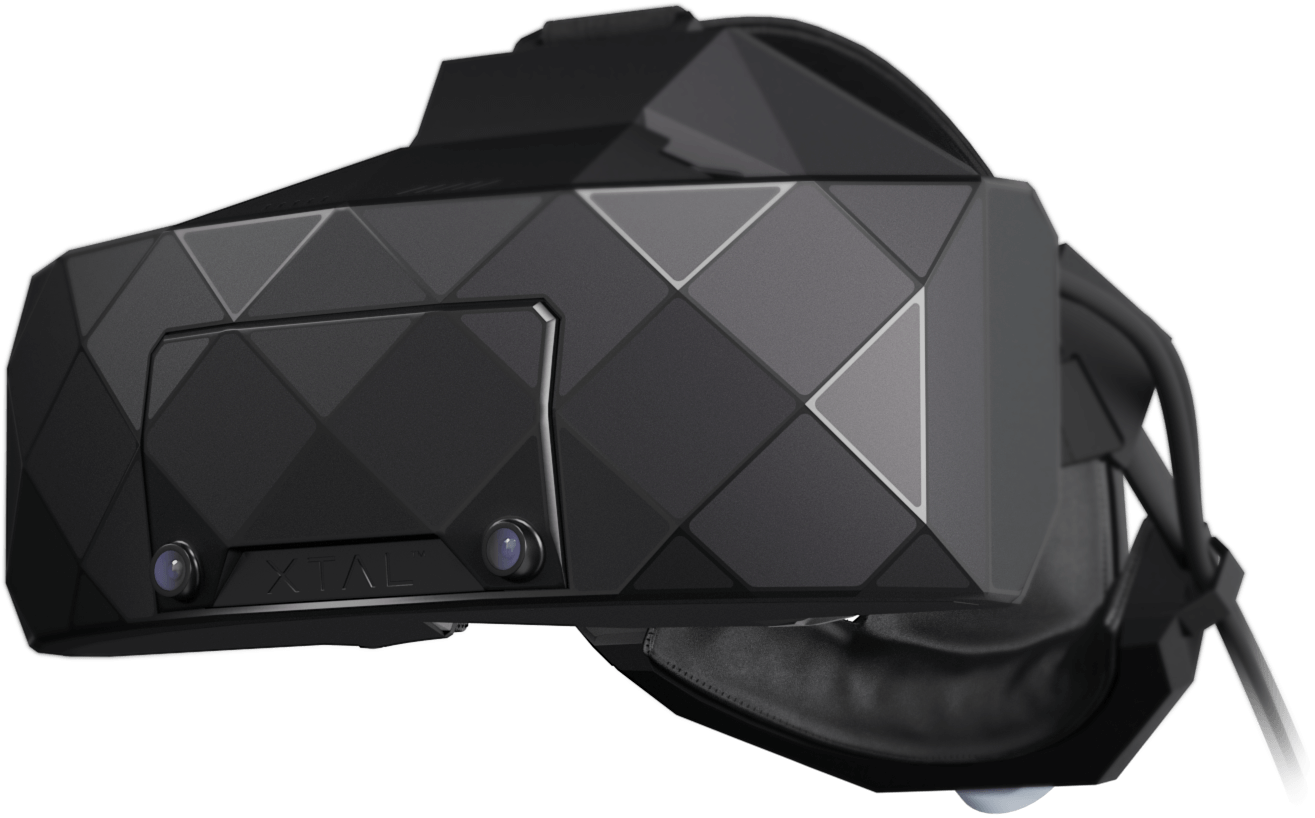
\includegraphics[width=0.6\textwidth]{img/xtal3.png}
    \caption[VRGineers XTAL 3 VR headset.]{VRGineers XTAL 3 VR headset.~\cite{vrgineers-xtal3-image}}
    \label{fig:vrg-xtal3}
\end{figure}

\subsubsection*{Eye tracker specification}
In this Bachelor's thesis written under the~Faculty of Electrical Engineering, CTU in 2020, a~prototype of eye detection and gaze estimation using the~ET system of the~XTAL headset was implemented. The~author used the~dark pupil method to~detect the~eyes by scanning the~pupil in the~recorded eye images. Gaze estimation was performed using a~2D regression method.~\cite{trnka2020thesis}

At this point, it is not clear whether the~ET implementation from the~Bachelor's thesis is present in the~current driver or if it has undergone significant changes. It is unrealistic to~assume the~accuracy of the~measuring algorithm because the~manufacturer has not yet provided it. 

ET does not work in XTAL without calibration. While a~VR application is running, one of the~two calibration options in the~VRG runtime must be triggered. The~faster one is the~one point calibration, which is used to~measure the~PID and enable foveated rendering, but can also be used to~enable ET itself. This option uses for calibration a~virtual mathematical model of the~user's face. For more accurate results of the~measured gaze data, the~more advanced calibration, consisting of seven points, should be used.~\cite{vrginners-xtal3-intro, vrginners-email}

\subsubsection*{XTAL VR Training}

Vrgineers has partnered up with the~U.S. Air Force to~build custom simulators for training fighter pilots. The~simulator can be seen in Figure~\ref{fig:vrg-cockpit}. When the~pilots sit inside, they have the~XTAL 3 XR headset on. This is an~example of VR training that mimics the~environment of various fighters such as F-15, F-18, and F-35 as closely as possible to~train muscle memory and situational awareness of pilots.~\cite{vrginners-classroom}


\subsubsection*{3D CAVE}
The~room with CAVE 3D is a~laboratory of the~Faculty of Mechanical Engineering of CTU. It consists of a~multiprojection system called CAVE, which is used to visualise scenes and scientific data. The~CAVE simultaneously projects stereoscopic images onto four cube faces; the~front, right, and left walls with the~floor, Figure~\ref{fig:cave-proj}. More specifically, it is used to display and verify virtual prototypes, where real physical parts of the~structures are compared to the~virtual prototype.~\cite{cave-lab}

The~very second part of this lab is a~corner with four XTAL headsets that run the~same application as the~projection system. The~headset can be walked around the~lab by attaching it to an~HP backpack. Figure~\ref{fig:cave-xtal}.

\begin{figure}[!ht]\centering
    \begin{subfigure}[b]{0.48\textwidth}
        \centering
        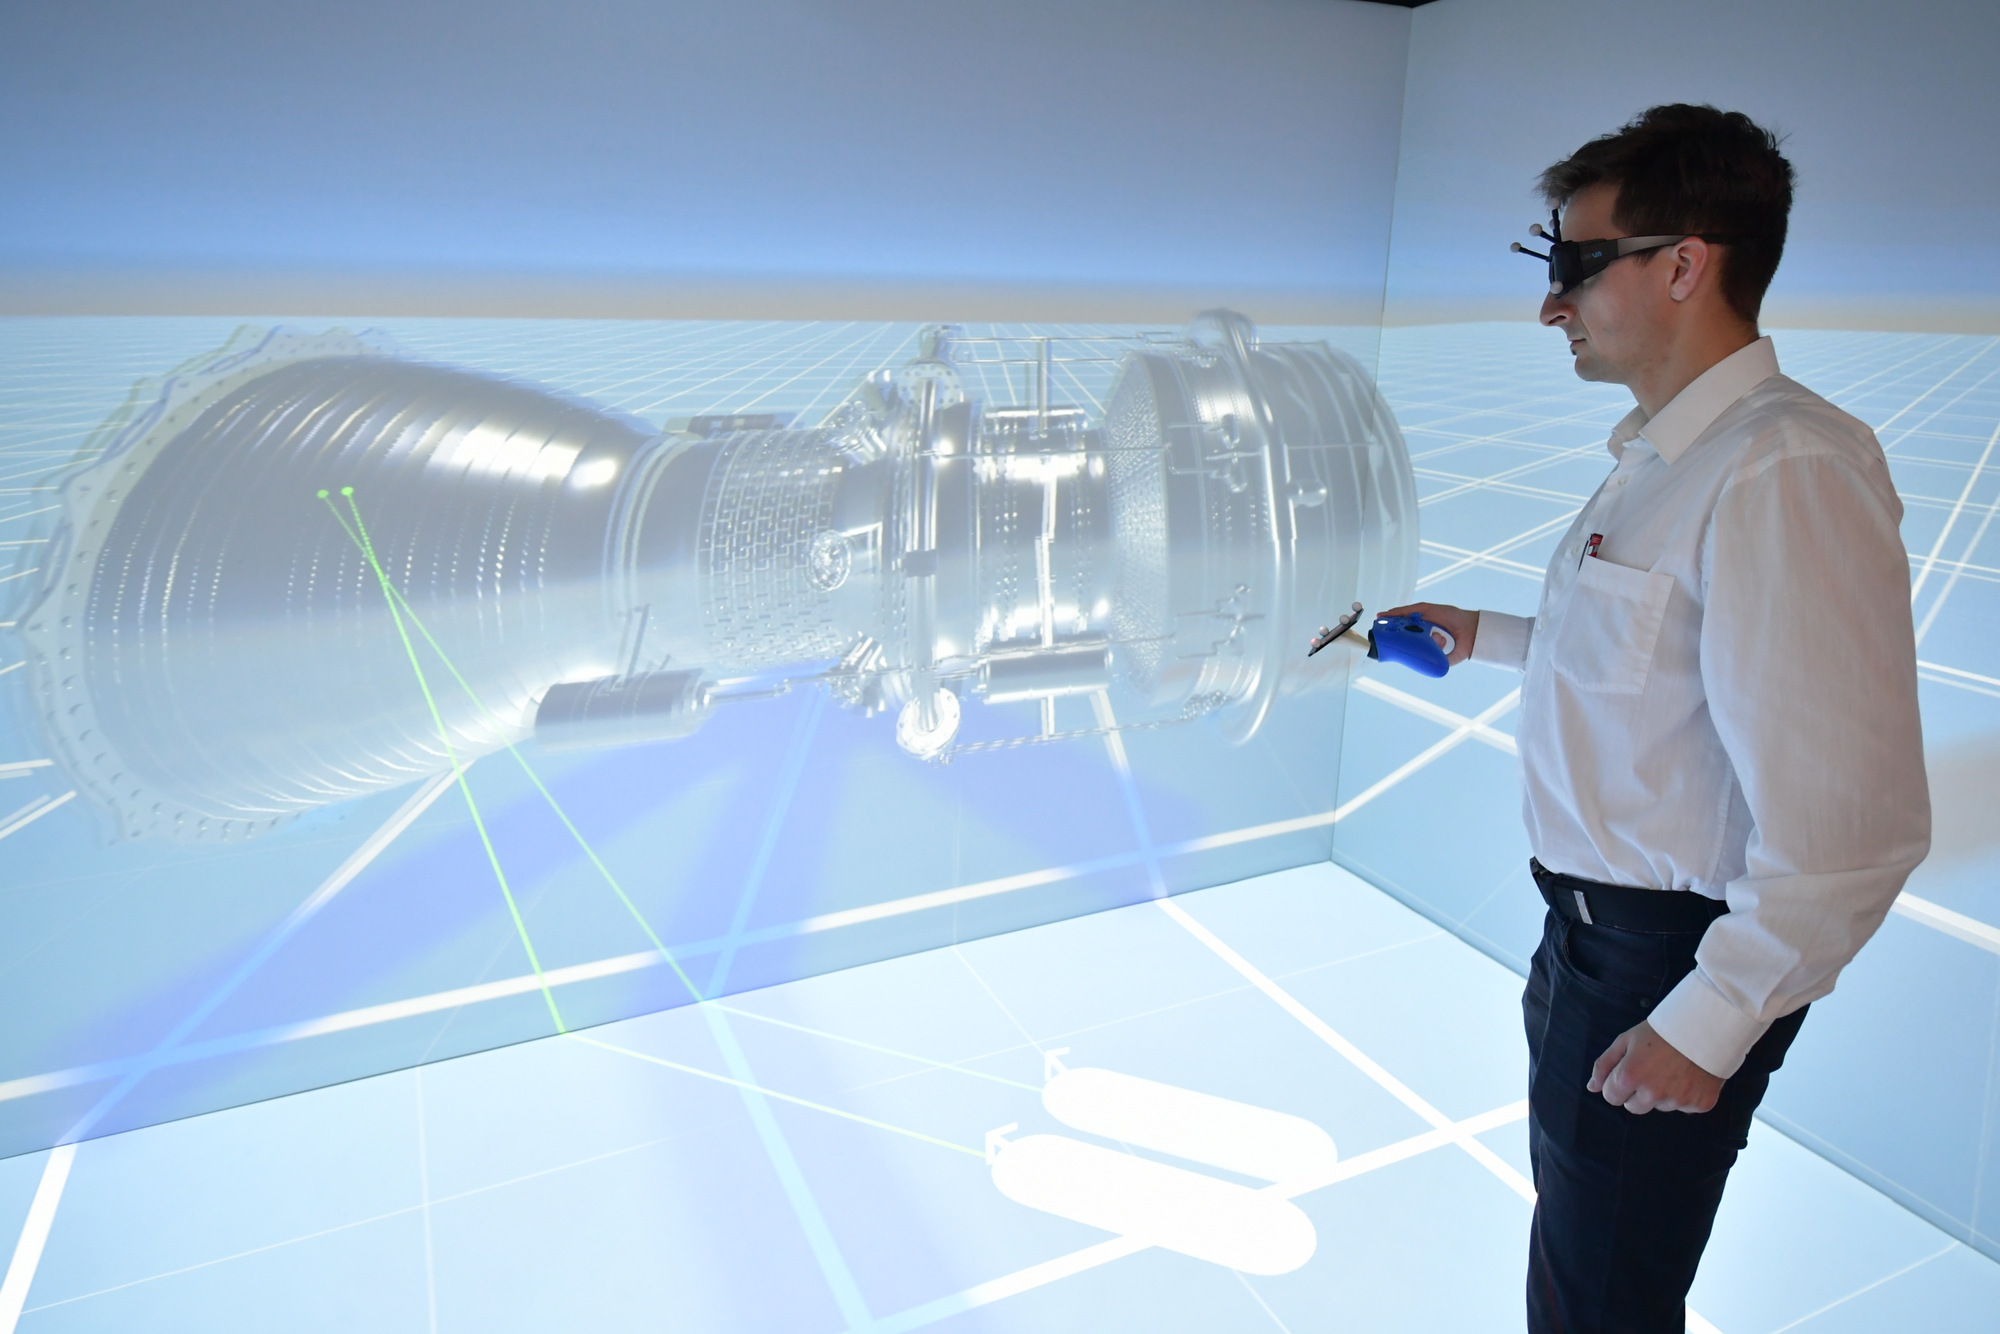
\includegraphics[width=\textwidth]{img/cave-projection.jpg}
        \caption{CAVE 3D multi-projection system.}
        \label{fig:cave-proj}
    \end{subfigure}
    \hfill
    \begin{subfigure}[b]{0.48\textwidth}
        \centering
        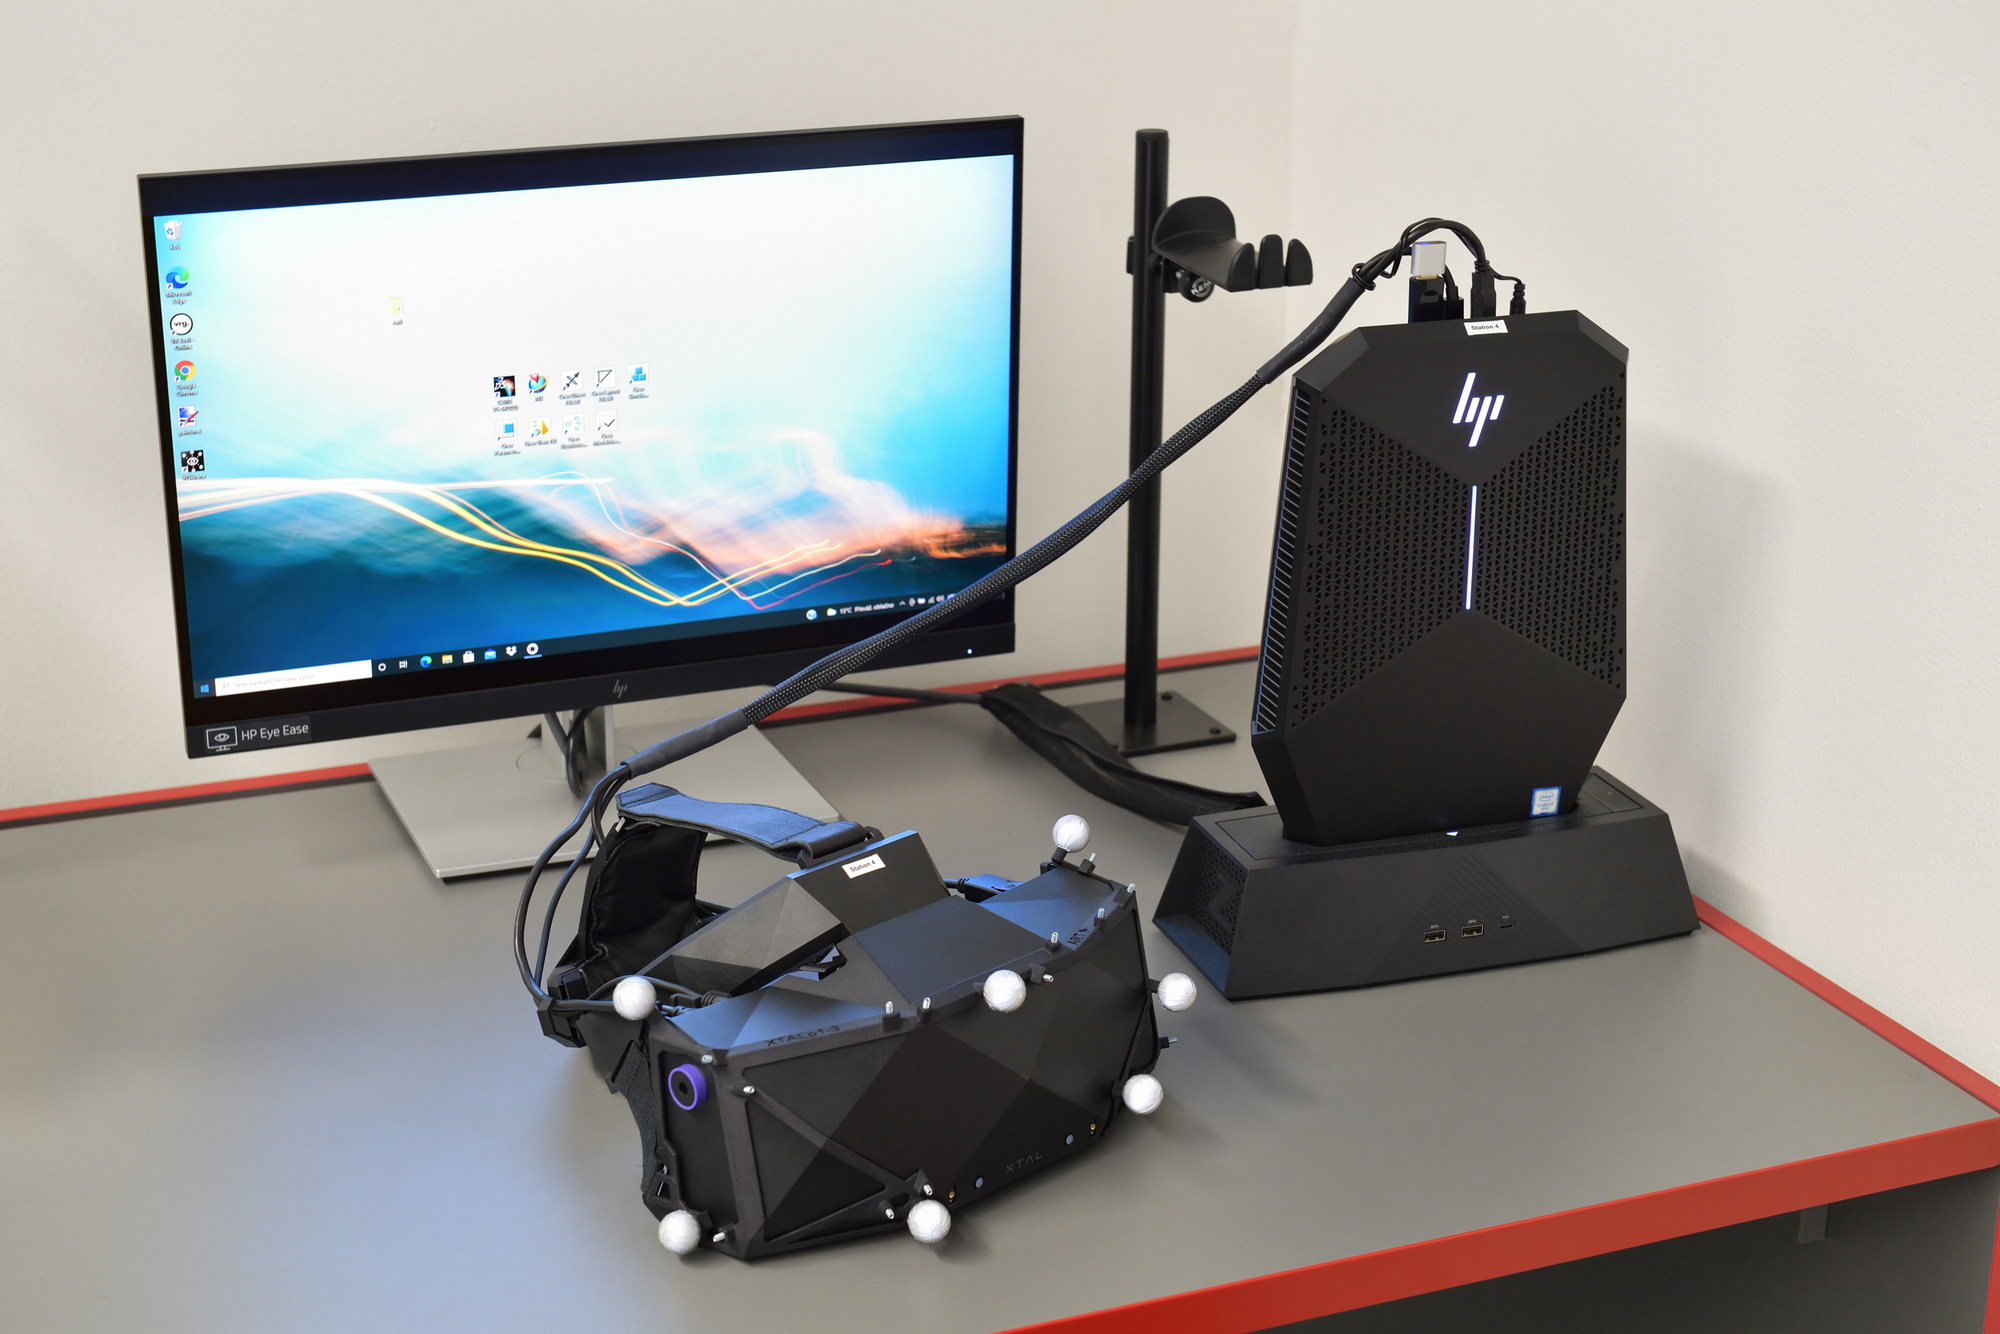
\includegraphics[width=\textwidth]{img/cave-xtal.jpg}
        \caption{XTAL with HP backpack.}
        \label{fig:cave-xtal}
    \end{subfigure}
    \caption[3D CAVE laboratory at CTU FME.]{3D CAVE laboratory at CTU FME.~\cite{cave-lab}}
\end{figure}


\begin{figure}[!ht]\centering
    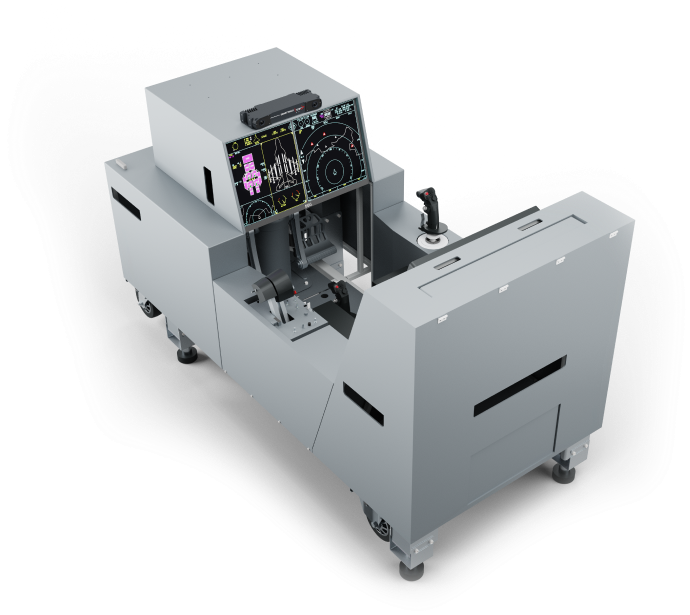
\includegraphics[width=0.5\textwidth]{img/xtal-cockpit.png}
    \caption[VRGineers fighter jet cockpit simulator.]{VRGineers fighter jet cockpit simulator.~\cite{vrgineers-cockpit}}
    \label{fig:vrg-cockpit}
\end{figure}

\subsection{Future possibility}

Another headset currently in development is the~successor to the~Playstation VR headset, which is designed for the~PS5 console; the~PSVR2. A~huge advantage of the~original version was that it was one of the~most affordable VR headsets on the~market. It admittedly did not have the~best specifications, but it did not cost more than \$400 when it was released. Compared to the~other headsets that could be purchased for at least double that amount. Although the~headset was made to be used exclusively on a~Playstation platform, it is possible to~communicate with it on a~PC via unofficial drivers.

The~new PSVR2 has dramatically improved technical specifications over its predecessor. The~internal OLED panel offers 2000x2040 pixels for each eye with a~refresh rate of up to 120~Hz, and an~FOV of 110 degrees. Most interestingly, it includes an~eye tracker. Sony's implementation will likely be proprietary to~keep the~cost as low as possible. The~setup is conventional with IR illuminators and one IR camera for each eye. The~main reason they want to~implement ET is to~add additional input for new games and for the~foveated rendering capability, which is mainly to~free up PS5 rendering performance. It~should offer developers of new PSVR games access to the~same gaze data structure as the~previous ET headsets.~\cite{psvr2, psvr2-specs}

Sony has not yet announced the~price of the~PSVR2 at the~time of writing this thesis, but it is rumoured that it will be around the~retail price of PS5, which based on the~announced specifications would be a~great bargain. The~question is whether Sony will develop an~official PC driver for it, or if there will be an~unofficial one that will for example communicate with this headset according to the~OpenXR standard. If so, the~headset would become the~cheapest VR headset with ET on the~market capable of being used for ET research.

\section{Existing solutions}
\label{sec:solutions}

This section summarises the~available solutions that use a~VR headset to~collect and visualise ET data with the~requirement of using game engines. Given how advanced modern ET hardware is, the~number of software implementations that use it is scarce. The~main player is Cognitive3D, which was the~first to~produce a~robust solution that addresses this and does so using current game engines.

The~Master's thesis written at the~Faculty of Informatics of Masaryk University in 2020 explored the~possibilities of ET technology in the~context of VR, where the~student designed and implemented a~software solution to~record, analyse, and visualise gaze data in~Unity with the~use of the~HTC VIVE Pro Eye headset for VR~\cite{ugwitz2020thesis}. The~solution was used for a~user study exploring escape behaviour. The~student did not evaluate the~gaze data in real time but first collected them into an~external CSV file, which was later analysed. To~visualise these data, he used visual indicators that were assembled from basic Unity primitives such as a~cube, a~sphere, or a~lineRenderer. Points of fixation (PoF) are visualised in the~thesis as concentrations of several ET points in a~3D space, which are coloured by a~white-to-pink gradient that is supposed to~liken them to~heatmaps.

\subsection{Cognitive3D}
Cognitive3D is a~company based in Vancouver, Canada, that offers an~entire proprietary system made up of several parts for the~collection and analysis of ET data. The~system includes a~streamlined production of use-case scenarios that are defined using objectives. The~system can also be used for VR environments that do not employ ET in any way. It~is applicable to~academic and marketing research, VR training simulation, or architectural design. It~has been designed to~allow any content from Unreal or Unity to~be integrated into the~system using the~corresponding \emph{plug-in}. The~\emph{plug-in} takes control of the~entire scene in an~engine. The~annual academic licence is in the~range of tens of thousands of dollars.~\cite{cognitive3d-splash, cognitive3d-meeting}

\pagebreak{}


% \begin{figure}[!ht]\centering
%     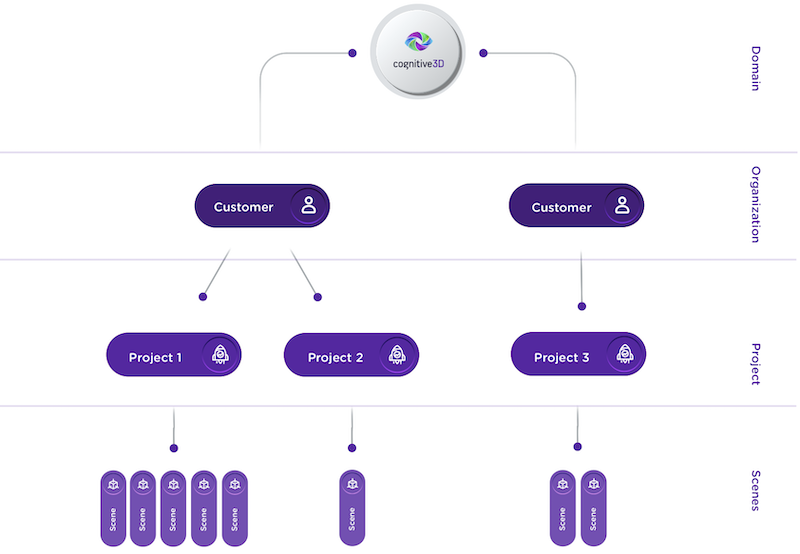
\includegraphics[width=0.8\textwidth]{img/cognitive3D-platform-hierarchy.png}
%     \caption[Cognitive3D platform hierarchy.]{Cognitive3D platform hierarchy.~\cite{cognitive3d-dashboard-concepts}}
%     \label{fig:cognitive3d-platform}
% \end{figure}

\subsubsection*{Dashboard}
The~application that holds the~whole platform together is called Dashboard. It is a~web interface that contains several different functions and handles the~structure of multiple users/organisations and their projects.~\cite{cognitive3d-dashboard-concepts}

A~\emph{customer} is an~entity with a~paid licence that can create various projects. Each \emph{project} can have multiple defined \emph{scenes}, which are containers for static scene geometry, \emph{dynamic objects} and \emph{session} data. A~\emph{session} is a~specific instance of a~single participant measurement that collects session data during the~runtime of a~Cognitive3D application that contains a~scene of an~experiment.

\subsubsection*{SceneExplorer}
One of the~main functions of the~Dashboard is the~SceneExplorer, which is used for a~detailed review of the~participant's session. This session contains a~timeline that stores all actions, events, user movements and gazes, and fixations on objects performed during an~experiment. The~timeline can be stopped at any time to~explore the~state of the~scene. It can display exactly where the~participant was looking. The~gaze is visualised as a`heatmap that fades according to a~time fall-off. Fixation points are displayed using a~trail consisting of spheres (fixations) and lines (saccades).~\cite{cognitive3d-scene-explorer}

\subsubsection*{Gaze and Fixations}
Cognitive3D can be used without an~ET headset, but in this case fixations and their metrics cannot be collected during the~experiment, only gaze, which is collected based on the~virtual position of the~HMD. Gaze metrics are recorded always, but without an~eye tracker the~application assumes that the~participant's focus is directly in front of the~HDM. In this case, the~metrics are significantly less accurate.~\cite{cognitive3d-unreal-gf}

\begin{table}[!ht]
\begin{tabular}{|c|l|}
\hline
Metric &
  Description \\ \hline\hline
\begin{tabular}[c]{@{}c@{}}Average Gaze Count\end{tabular} &
  \begin{tabular}[c]{@{}l@{}}The~average number of times someone gazed at the~object during\\ one session.\end{tabular} \\ \hline
\begin{tabular}[c]{@{}c@{}}Average Gaze Time\end{tabular} &
  \begin{tabular}[c]{@{}l@{}}The~average time the~object was gazed at during one session.\end{tabular} \\ \hline
Gaze Ratio &
  \begin{tabular}[c]{@{}l@{}}Reports the~percentage of sessions in which the~object was gazed at.\end{tabular} \\ \hline
\begin{tabular}[c]{@{}c@{}}Total Sessions\\ with Object\end{tabular} &
  \begin{tabular}[c]{@{}l@{}}The~number of times the~object was present in a~session.\end{tabular} \\ \hline
\begin{tabular}[c]{@{}c@{}}Total User Gazes\\ at Object\end{tabular} &
  The~total number of all gazes. \\ \hline
\begin{tabular}[c]{@{}c@{}}Sessions with\\ Gaze\end{tabular} &
  \begin{tabular}[c]{@{}l@{}}The~number of sessions in which the~participant noticed the~object\\ at least once.\end{tabular} \\ \hline
User Gaze Length &
  The~total duration of all gazes. \\ \hline
\begin{tabular}[c]{@{}c@{}}Gaze Instance\\ Duration\end{tabular} &
  The~average duration of one instance of gaze. \\ \hline\hline
Gaze Sequence &
  The~sequence of all objects that were seen earlier. \\ \hline
Time to Gaze &
  \begin{tabular}[c]{@{}l@{}}The~duration from the~beginning of the~session to the~first gaze of\\ the~object.\end{tabular} \\ \hline
\end{tabular}
\caption[Cognitive3D gaze metrics of dynamic objects.]{Cognitive3D gaze metrics of dynamic objects.~\cite{cognitive3d-metrics}}
\label{tab:cognitive3d-metrics}
\end{table}

\pagebreak{}

\begin{table}[!ht]
\centering
\begin{tabular}{|c|l|}
\hline
Metric &
  Description \\ \hline\hline
Completions &
  The~number of users that completed the~step. \\ \hline
\begin{tabular}[c]{@{}c@{}}Completions in \%\end{tabular} &
  \begin{tabular}[c]{@{}l@{}}Total number of completions compared to\\ the~total amount of sessions.\end{tabular} \\ \hline
\begin{tabular}[c]{@{}c@{}}Average Step Duration\end{tabular} &
  \begin{tabular}[c]{@{}l@{}}The~average time to complete the~step relatively to\\ the~previously completed step.\end{tabular} \\ \hline
\begin{tabular}[c]{@{}c@{}}Average Step\\ Completion Time\end{tabular} &
  \begin{tabular}[c]{@{}l@{}}The~average time to complete the~step relatively to\\ the~session start.\end{tabular} \\ \hline\hline
\begin{tabular}[c]{@{}c@{}}Successful Sessions\end{tabular} &
  \begin{tabular}[c]{@{}l@{}}Total number of sessions that have cleared\\ successfully every step.\end{tabular} \\ \hline
Total Sessions &
  \begin{tabular}[c]{@{}l@{}}Total amount of sessions with the~same objective.\end{tabular} \\ \hline
\begin{tabular}[c]{@{}c@{}}Success Rate in \%\end{tabular} &
  \begin{tabular}[c]{@{}l@{}}The~total number of successful sessions compared to\\ total sessions.\end{tabular} \\ \hline
\end{tabular}
\caption[Cognitive3D metrics used for objectives and its steps.]{Cognitive3D metrics used for objectives and its steps.~\cite{cognitive3d-metrics}}
\label{tab:cognitive3d-obj-metrics}
\end{table}

Gaze and fixation metrics are aggregated for individual dynamic objects that represent regions of interest (RoIs) in the~scene. A~group of several objects can be defined and treated as a~separate RoI. Both metrics have the~same structure, but their description is presented only on~gaze metrics~\cite{cognitive3d-dynamic-objects}. The~Table~\ref{tab:cognitive3d-metrics} shows gaze metrics that are collected for each object independently over all sessions of a~given scene. The~last two metrics are collected only in the~context of a~single session.~\cite{cognitive3d-metrics}

\subsubsection*{Objectives}

The~next main functionality of the~Cognitive3D software are the~objectives, which are composed of individual steps and thus represent a~certain script of what should occur during a~session. They allow to~collect information about what the~participant was able to~complete within a~session or if they followed a~certain process. Any~amount of objectives can be defined in the~context of a~scene, and any amount of these objectives can be assigned to a~session. An~example of one with a~list of individual steps and their calculated results in the~Dashboard web interface can be seen in Figure~\ref{fig:cog3d-steps}, and Figure~\ref{fig:cog3d-obj} displays the~dialogue box in which the~criteria of a~single step for its completion are set.~\cite{cognitive3d-objectives}

\begin{figure}[!ht]\centering
    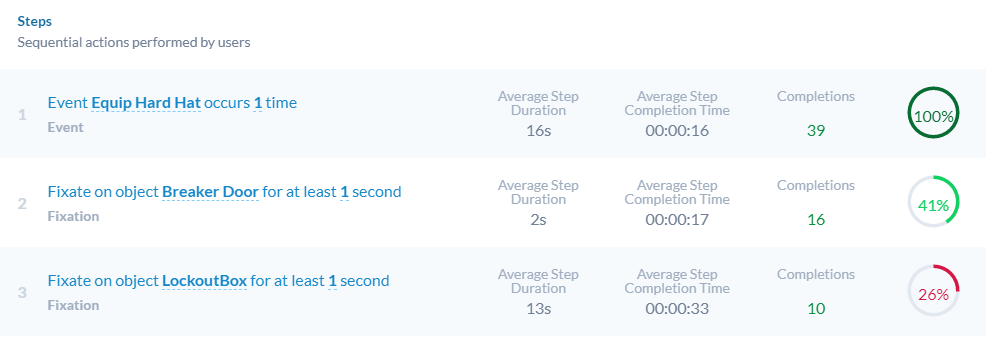
\includegraphics[width=\textwidth]{img/cognitive3D-steps.png}
    \caption[Sequence of steps and their completion in Cognitive3D.]{Sequence of steps and their completion in Cognitive3D.~\cite{cognitive3d-objectives}}
    \label{fig:cog3d-steps}
\end{figure}

\pagebreak{}
Registering whether a~step was successful can be easily evaluated using ET by whether the~participant fixated or gazed at a~particular object. A~step of an~objective is considered to be completed if it meets the~specified criteria. It is possible to set the~number of required fixations or their duration. Using this input, the~first four metrics shown in Table~\ref{tab:cognitive3d-obj-metrics} are collected for each step; the~same metrics can be seen in Figure~\ref{fig:cog3d-steps}. The~remaining three metrics of Table~\ref{tab:cognitive3d-obj-metrics} are collected for the~objective as a~whole. 

\begin{figure}[!t]\centering
    \includegraphics[width=0.7\textwidth]{img/cognitive3D-objective.png}
    \caption[Setup of a~step in Cognitive3D that activates at gaze.]{Setup of a~step in Cognitive3D activating at gaze.~\cite{cognitive3d-objectives}}
    \label{fig:cog3d-obj}
\end{figure}

\subsubsection*{Supported hardware}
The~system is built to~be compatible with a~wide range of devices. It offers a~high number of VR devices without ET. Among the~VR HMDs with ET, it supports all of the~previously mentioned with Tobii eye tracker in Section~\ref{sec:integrations} and all Varjo headsets in Section~\ref{sec:varjo}. Support for XTALs did not exist during the~writing of the~thesis.

\section{Unreal Engine capabilities}

\emph{Unreal Engine} (UE), developed by Epic Games~\cite{unreal-engine}, is used to render 3D computer graphics in real time. First designed for game development, it has found use in many other industries. Engine development is possible in C\texttt{++} or using \emph{Blueprint Visual Scripting}. This section first briefly introduces the~tools used for development inside the~engine~\cite{unreal-documentation} and the~options on how to process gaze data for heatmap production in real time.

\subsection{Blueprint Visual Scripting}
\emph{Blueprint}, short for \emph{Blueprint class}, is based on a~node-based interface to create, modify, and control elements in an~Unreal scene. It is essentially a~class that is stored as an~Asset in the~Content Browser. It allows designers to use programming tools without having to touch the~C\texttt{++} language. 

Any functionality that Blueprints do not offer can be programmed using C\texttt{++} and then made available to Blueprint nodes. A~Blueprint does not have to contain a~functionality for a~specific gameplay element. It can exist fully independently as a~collection of static functions. It is called \emph{Blueprint Function Library}. Unreal Engine already comes with a~rich set of tools that define many Blueprint classes and libraries. Many Blueprint classes can be used as a~parent class for new ones that inherit their functionality.

\subsection{Tools and Classes}
For this thesis, it is crucial to know these UE options. The~scale of an~UE scene is defined in centimetres.

\begin{description}
    \item[Asset] is a~piece of content, the~engine can work with, that is located in Content Browser; part of Unreal's interface. Assets are files stored with \path{.uasset} extension. They represent, for instance, imported models and textures, or Blueprints.
    \item[Actor] is a~class that by default maintains 3D spatial information about its position and rotation, which can always be modified. An~Actor is spawnable and destroyable at any time. It can be, for example, a~controlled character, cameras, lights, or other 3D models. Each Actor in a~scene has its own Blueprint and a~\emph{Component graph}; hierarchical tree of Components.
    \item[Pawn] is an~Actor that is the essential physical representation of a~player within the~world. It is the~base class for all Actors that can be controlled either by a~player or an~AI. It is possible to add a~DefaultPawnMovementComponent to a~pawn to extend it with simple no-gravity movement.
    \item[Character] is a special type of Pawn that offers basic movement abilities for vertically orientated characters that can walk, run and jump.
    \item[Component] is a~Blueprint class that provides functionality that is attachable to any Actor at any time. 
    \item[Level] is a~special type of Asset that serves as a~hierarchical collection of several different Actors to create a~scene. Each Level in a~project has one Blueprint assigned by default.
    \item[Tick] is defined within the~engine as a~regular interval that usually occurs once every frame. An~actor may have a~defined OnTick function that is repeated periodically. It is often used to update a~given Actor.
    \item[Material] is an~Asset that defines how a~surface should be rendered. It is defined using visual scripting nodes -- Material Expressions -- in the~Material Editor, which is not a~Blueprint. Each material is translated as an~HLSL programme executed on a~GPU consisting of a~vertex and a~pixel shader. The~nodes replace pieces of HLSL code.
    \item[Static mesh] is an~object class that represents the~fundamental renderable static geometry. It is generated by importing a~3D model into a~UE project. It can be edited in the~Static Mesh Editor, which includes, among other functions, collision, UV map, and LOD settings or Material~assignment. A~static mesh also exists as a~Component or an~Actor, which effectively contains a~StaticMeshComponent as the~root of its graph. The~mesh is rendered according to the~assigned material.
    \item[Material Instancing] is a~method that is used to change the~appearance of material without recompiling the~HLSL programme. Some Material Expression nodes such as vectors, textures and floats can be turned into parameters that are set before the~Material is rendered. This requires to construct a~Dynamic Material Instance of the~given Material.
    \item[Canvas Render Target 2D] is a~Blueprint object class that inherits Texture class. This is a~texture that can be constructed, modified, and exported at runtime.
    \item[Scene Capture 2D] is a~camera Component that captures a~scene from its position using its view frustum into a~texture. It can record the~scene continuously every Tick or just once by calling its Blueprint function \emph{Capture Scene}.
    \item[ShowOnly List] is an~option inside the~Scene Capture Component's settings that allows to render only those objects that are in the~list. This option must be explicitly enabled first.
    \item[Line Trace] is a~Blueprint function, callable only from an~Actor, that will perform trace collisions along a~specified 3D line; parameters Start and End. The~function returns the~first object hit by this line.
    \item[Plug-in] is a~collection of code or data that developers can enable or disable within their projects. Additional plug-ins are installed by placing them in the~project's Plugins directory or the~UE root directory in the~[Root]/Engine/Plugins folder.
\end{description}

\subsection{OpenXR}
There are different ways to interact with VR, XR, and AR devices in Unreal. However, it offers a~unified way to access them using OpenXR. To activate certain features, it is crucial to enable a~certain plug-in. Basic compatibility is guaranteed by the~OpenXR plug-in. Additional functionality can be activated by enabling OpenXRHandTracking and OpenXREyeTracker.

Due to potential conflicts and errors, it is recommended to disable other proprietary plug-ins designed to communicate with their hardware and other methods such as SteamVR, OculusVR, or Oculus OpenXR.

Unreal offers a~simple interface for ET, through which gaze data from OpenXR are sent when the~plug-in is enabled. \emph{Get Gaze Data} returns a~combined gaze, \emph{Get Stereo Gaze Data} returns two gazes, one for each eye. The~gaze data structure consists of an~origin and direction vector in the~absolute real world coordinates of a~tracking system used with the~headset. 

\subsection{UV mapping}
A~static mesh is a~geometric shape that remains unchanged and always contains the~same number of vertices and faces. The~way static meshes are rendered depends on their attached Material. Often these meshes are rendered with a~texture according to their UV maps.

\emph{UV mapping} is a~procedure in which a~2D image is projected onto a~3D model. For this to happen, it is necessary that the~3D model has its own UV map, which assigns to its vertices its own $(u, v)$ coordinate where $u,v$\,$\in$\,$[0, 1]$. A~texture or an~image has its width and height scaled to the~range of the~UV map during rendering. The~areas formed by connecting the~$(u, v)$ coordinates of the~vertices project the~corresponding piece of a~texture onto the~3D mesh itself.

\pagebreak{}
\subsection{Mesh painting}

Unreal offers the~ability to create dynamic textures using Render Targets and Dynamic Materials. Drawing on the~mesh itself can be simulated by modifying its texture. For this to work, the~UV map must not have overlapping faces defined. Each face of the~3D model must have a~uniquely assigned area in the~texture. This is also required by lightmaps in UE, which are used to bake scene lights into textures themselves, so they do not have to be computed during rendering.

In the~context of ET data visualisation, there is the~question of using mesh painting to produce heatmap textures based on a~gaze vector that collides with the~given object. Render Target can be exported in runtime.

It needs to be tested if this method of data collection is worth doing in real-time performance-wise, and how much storage it will require with multiple objects in the~scene -- each must have its own heatmap texture.

\subsection{UV painting method}

The~first approach to drawing heatmaps on textures would be to use a~collision hit position of the~object, which will be mapped to the~appropriate $(u, v)$ coordinate. This requires enabling the~Support UV From Hit Results option in the~Engine -- Physics section of the~UE project settings. 

This Unreal tutorial~\cite{texture-painting-tutorial} shows a~method for painting with a~brush defined using a~Material, which is set to additive blend mode. This is necessary to add new values to the~resulting Render Target instead of replacing them. 

\begin{figure}[!ht]\centering
    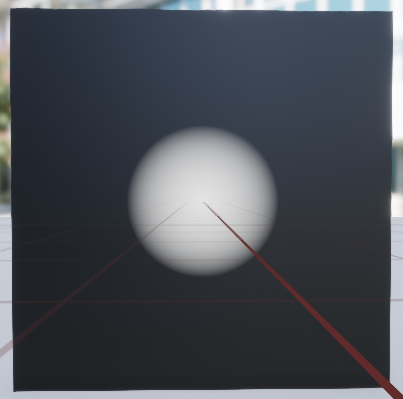
\includegraphics[width=0.4\textwidth]{img/Brush-material.png}
    \caption[Preview of 2D brush Unreal Material.]{Preview of 2D brush Unreal Material.~\cite{basic-heatmap-tutorial}}
    \label{fig:brush-material}
\end{figure}

The~brush material is shown in Figure~\ref{fig:brush-material}. The~appearance of the~preview corresponds to the~brush settings of $0.2$ radius and $(0.5, 0.5)$ coordinate on an~UV map. The~material has these values as input parameters that can be set before rendering to a~Render Target. As these parameters change, the~brush will change its position and size.

Render Target must be a~square texture that directly shadows the~UV map range. This texture is set to a~16-bit colour depth for each channel for greater detail of the~brush.

It is beneficial to first record the~heatmap as a~brush trail for easier manipulation of the~visualisation. One material can be seen in this Unreal tutorial~\cite{basic-heatmap-tutorial}. The~recorded trail can be displayed as a~heatmap on a~model using additional material that will be responsible for its appearance. The~parameters of the~Material are set by its Material Blueprint functions with the~wording \emph{Set Parameter Value}. A~Material is rendered to a~Render Target using the~Blueprint function \emph{Draw Material To Render Target}.

\subsubsection*{Problems}
There is however a~major drawback to this method. Brush splats are always drawn directly on a~texture. It does not reflect the~actual geometry and size of the~3D model in the~scene. The~UV map is not guaranteed to have all faces defined on the~same scale or aspect ratio. For such models, this would cause the~heatmap trail to be stretched for some faces or to be of a~different size. 

For symmetric, uniform, and unambiguous models with a~clearly defined UV map, such as a~cube or a~plane, this will certainly work much better. But it is also inadequate because it does not prevent brush overflow, where the~drawing stroke on a~certain face overflows into another. An example of this issue is demonstrated in the \path{video/01-basic-painting-method.mp4} in the enclosed DVD. The~wall model in the~video is a~single object. This solution is unsatisfactory and a~more suitable one is needed to address these problems.

\subsection{UV unwrap method}
\label{sec:uv-unwrap-method}

In this blog post~\cite{brucks2016shaderbits}, Unreal Engine veteran Ryan Brucks discusses automatic UV dilation to prevent edge bleeding for lower resolution mipmaps. In the~process, he also published his method for unwrapping meshes on the~basis of its UV map. The~first step in achieving dilation involves unwrapping the~model in the~world according to UV. The~object appears in the~scene as a~3D plane, which is rendered using an~orthographic Scene Capture Component to a~Render Target with a~32-bit pixel depth. In this texture, 3D coordinates of the~mesh's absolute position in the~world are captured. 

Dilation is then achieved by stretching the~faces' edges on the~UV map using algorithms that make use of other UE Materials. What is needed mainly for this thesis is the~unwrap method. Use a~brush that imprints itself on the~texture in the~exact areas around where a~gaze vector has hit the~object.

This requires using the~absolute world coordinates of the~mesh vertices while arranging the~vertices of an~object to appear on a~single unwrap plane that will be recorded in a~texture. The~way a~model looks when it is unwrapped can be seen in Figure~\ref{fig:unwrapped-mesh}, and how it is implemented in the~Material Expression nodes is shown in Figure~\ref{fig:unwrap-offset}. 

\begin{figure}[!ht]\centering
    \begin{subfigure}[b]{0.48\textwidth}
        \centering
        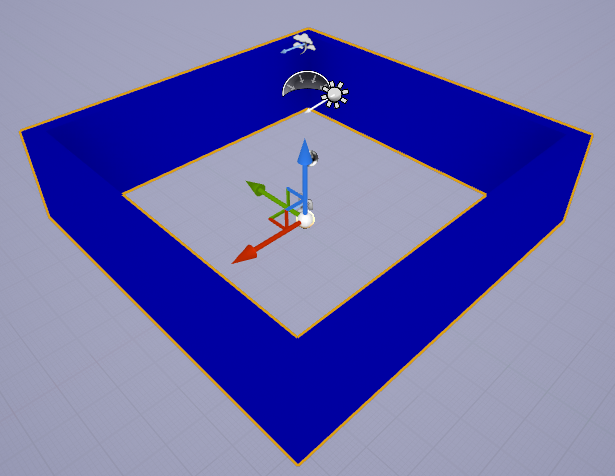
\includegraphics[width=\textwidth]{img/unwrap-method-original-mesh.png}
        \caption{Wall mesh.}
    \end{subfigure}
    \hfill
    \begin{subfigure}[b]{0.48\textwidth}
        \centering
        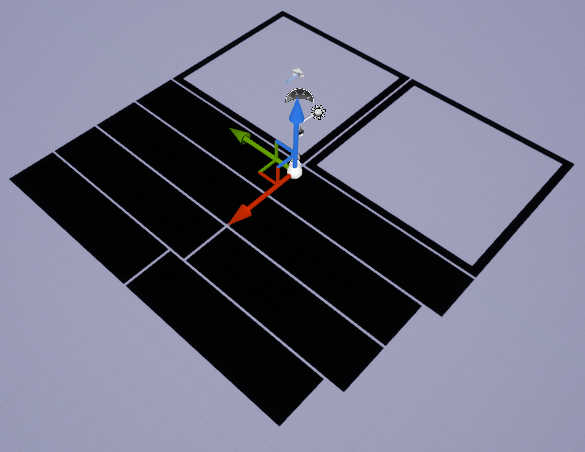
\includegraphics[width=\textwidth]{img/unwrap-method-mesh.png}
        \caption{Unwrapped wall mesh.}
    \end{subfigure}
    \caption{Difference between applied unwrap material.}
    \label{fig:unwrapped-mesh}
\end{figure}

\pagebreak{}
The~result of this algorithm is a~3D vector that is plugged into the~\emph{World Position Offset} pin in Material's result node, which is added to the~total World Position value of a~vertex. The~algorithm consists of creating a~plane in world coordinates from which the~absolute world position is subtracted, so that the~resulting shape is the~desired unwrap plane.

\emph{CaptureSize} parameter specifies the~size of the~square texture in which it will be rendered. For a~2048px texture, a~plane of size $20.48$ metres will appear in the~world, because the~scale of Unreal is in centimetres. This must be set to always add the~correct values to the~texture. 

\emph{UnwrapLocation} vector parameter moves the~centre of the~unwrap plane in the~world. Objects can reside at different locations in the~scene, and hard assigning values to the~scene's origin can cause problems. It may happen that object values are going to be recorded in an~unwrapped state and nothing will be added to the~texture. This is simply caused by the~object having been culled during the~rendering. The~actual position of the~object is somewhere else in the~scene, outside of a~view frustum range.

\begin{figure}[!t]\centering
    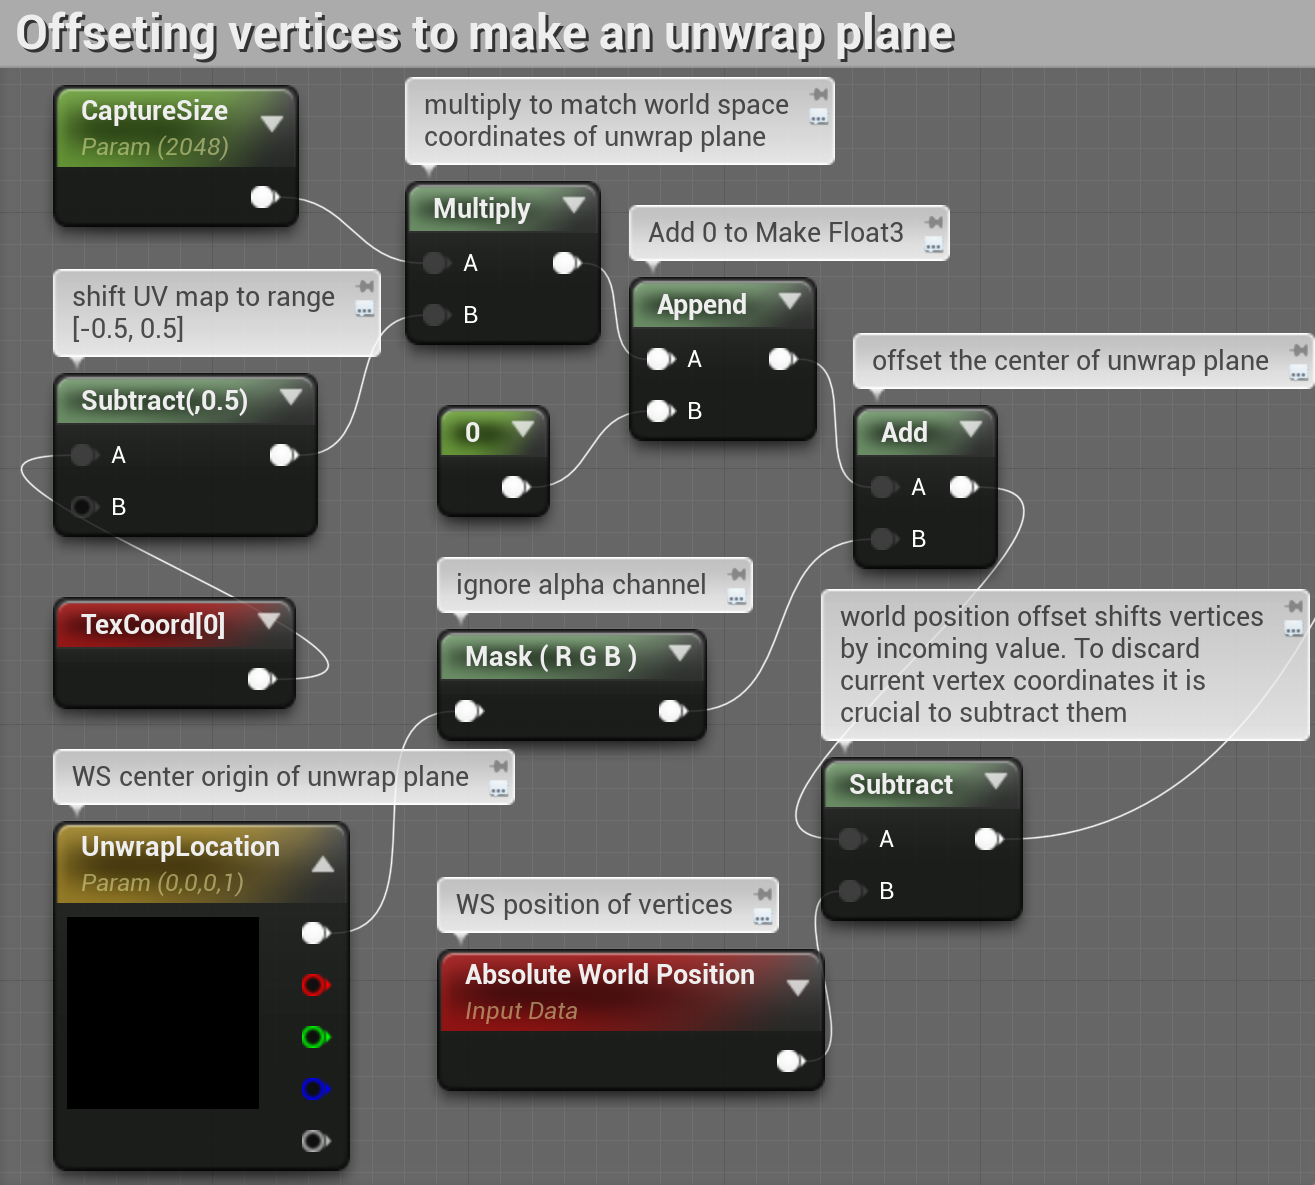
\includegraphics[width=\textwidth]{img/unwrap-method-nodes.png}
    \caption[Material Expressions used to unwrap mesh to world space.]{Material Expressions used to unwrap mesh to world space.~\cite{brucks2016shaderbits}}
    \label{fig:unwrap-offset}
\end{figure}

\pagebreak{}
\subsubsection*{Modification}
Tran proposes a~modification to this method~\cite{tran2018wenderlich} by not storing the~position in an~assistive Render Target, but creating a~3D brush in the~same Material that essentially does the~same thing as the~simpler method. Instead of comparing the~$(u, v)$ coordinate of the~hit location and the~$(u, v)$ coordinate of a~pixel, it compares the~hit location to the~pixel's absolute world position without Material offsets applied. The~implementation can be seen in Figure~\ref{fig:unwrap-3d-brush} which computes the~resulting colour that is supplied to the~Emissive Colour of the~Unwrap Material.

\medskip{}
\emph{BrushSize} parameter specifies the~size of the~3D brush radius. \emph{Strength} parameter determines how hard the~brush imprints on a~texture. It must be in the~range [0, 1]. A~value of 1 would create the~maximum value on the~heatmap and 0 would not make any changes.

\medskip{}
Now the~object is coloured based on a~3D brush that takes into account the~absolute position of the~mesh in the~scene. This method eliminates all the~problems that the~simpler method had.

\medskip{}

Tran's tutorial also offers a~basic Blueprint setup for recording this UV unwrap material using a~Scene Capture Component and a~black projection plane. For more information on the~implementation, see Section~\ref{sec:uv-unwrap-implementation}

\begin{figure}[!ht]\centering
    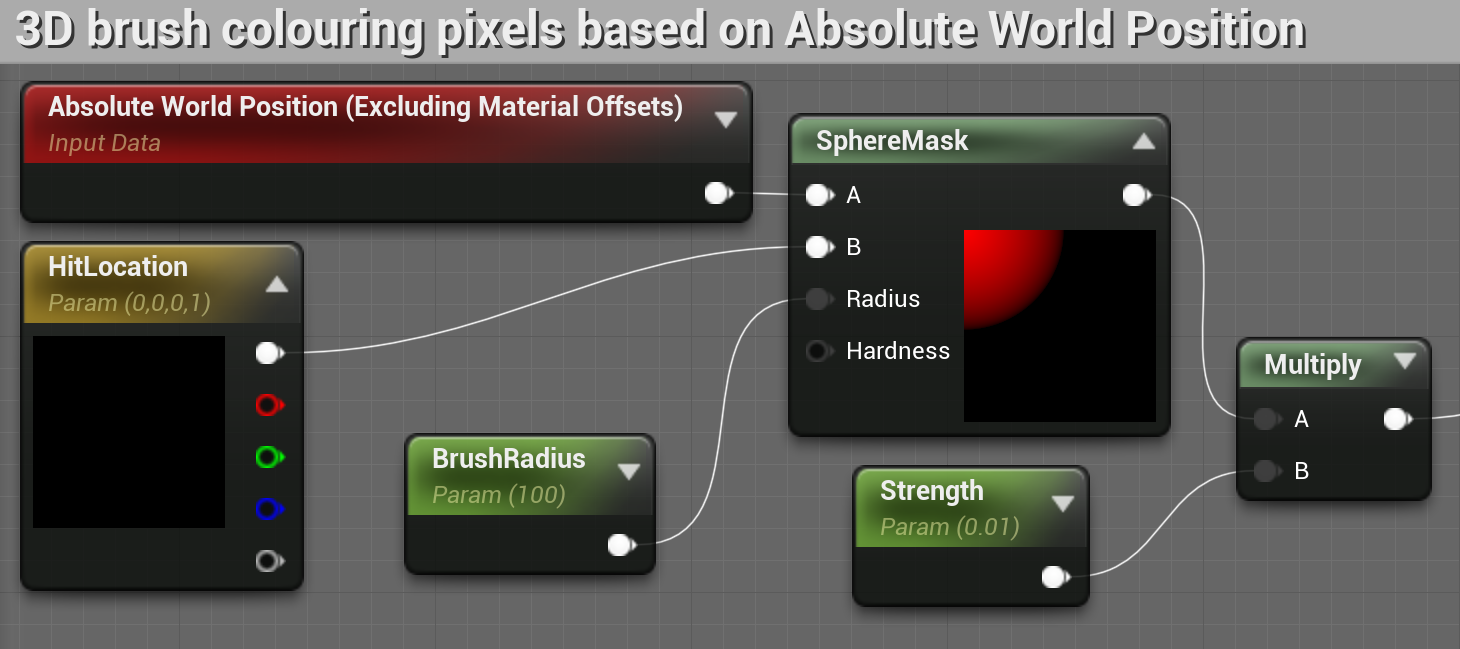
\includegraphics[width=\textwidth]{img/unwrap-method-3d-brush.png}
    \caption{3D Brush defined in Material Expressions.}
    \label{fig:unwrap-3d-brush}
\end{figure}

\subsection{Runtime texture loading}
\label{sec:texture-loading}

Exporting a~Render Target is simple, all it requires is a~single function called \emph{ExportToDisk}. The~function takes a~Texture Object reference, which is the~parent of the~Render Target, a~path with a~filename, and export options. Importing a~texture directly into the~Render Target is more complicated, as no such function exists. It is necessary to obtain the~assistance of a~material shown in Figure~\ref{fig:load-material}. The~process is shown in this tutorial~\cite{texture-loading-tutorial}.

Texture loading options exist, but only as a~Texture 2D object. This is done by the~\emph{Import File as Texture 2D} function, which takes a~file path as input. The~whole method is to redraw the~loaded texture into a~Render Target. Load Material does exactly that; it just sets the~texture parameter itself as the~output colour of the~material. This parameter must be set from the~Dynamic Material Instance by calling its Blueprint function Set Texture Parameter Value -- Figure~\ref{fig:unreal-texture-loading}. The~input value for this function is the~loaded texture, and the~Parameter Name. That must be the~same as the~Param2D name in the~Material.


\begin{figure}[!ht]\centering
    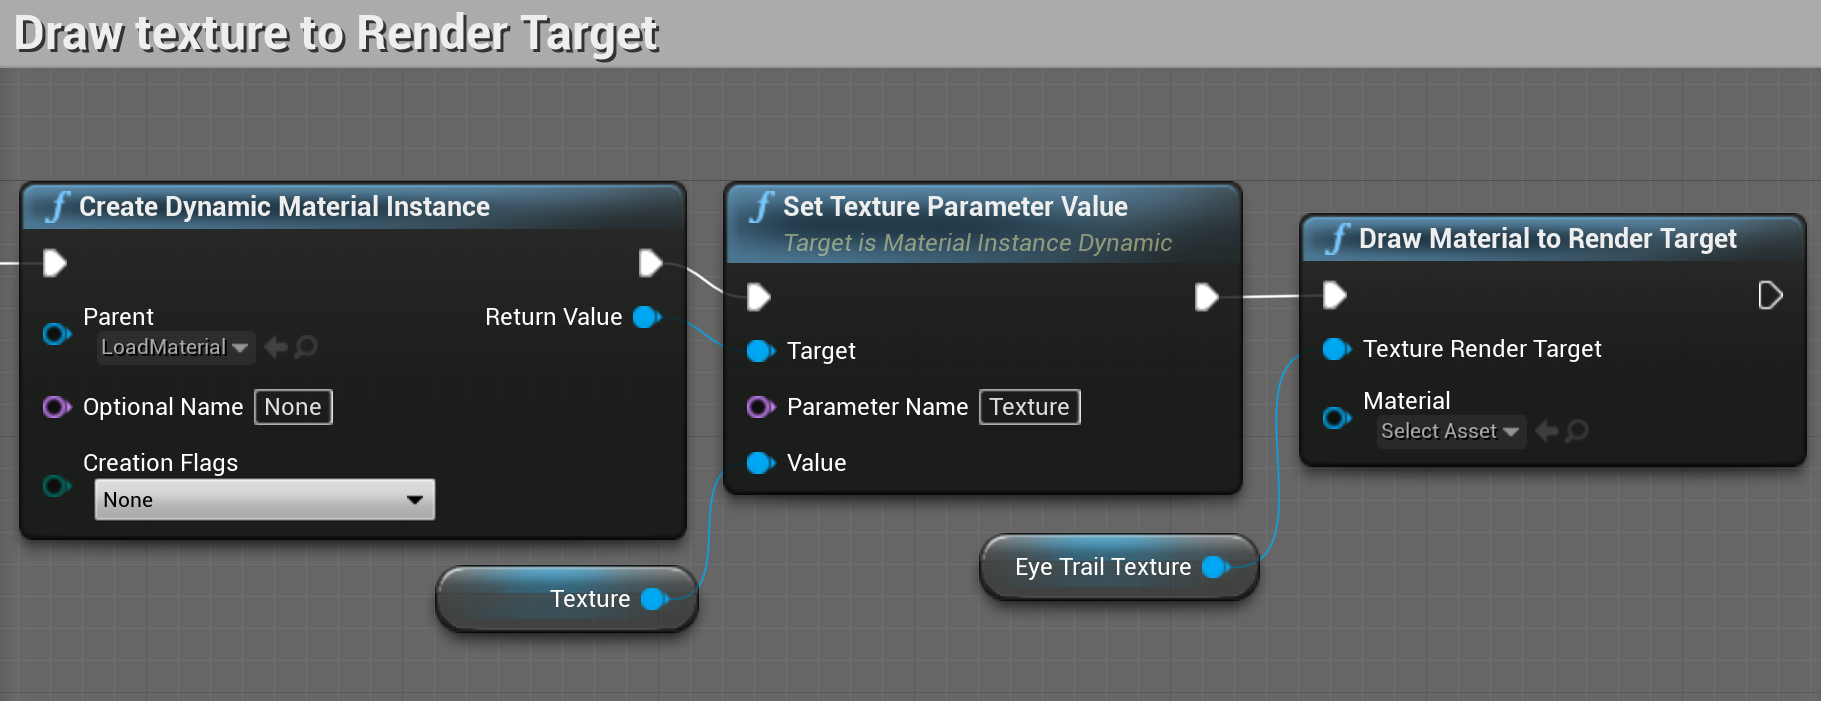
\includegraphics[width=\textwidth]{img/texture-loading.png}
    \caption{Process of importing texture on Render Target.}
    \label{fig:unreal-texture-loading}
\end{figure}

\begin{figure}[!ht]\centering
    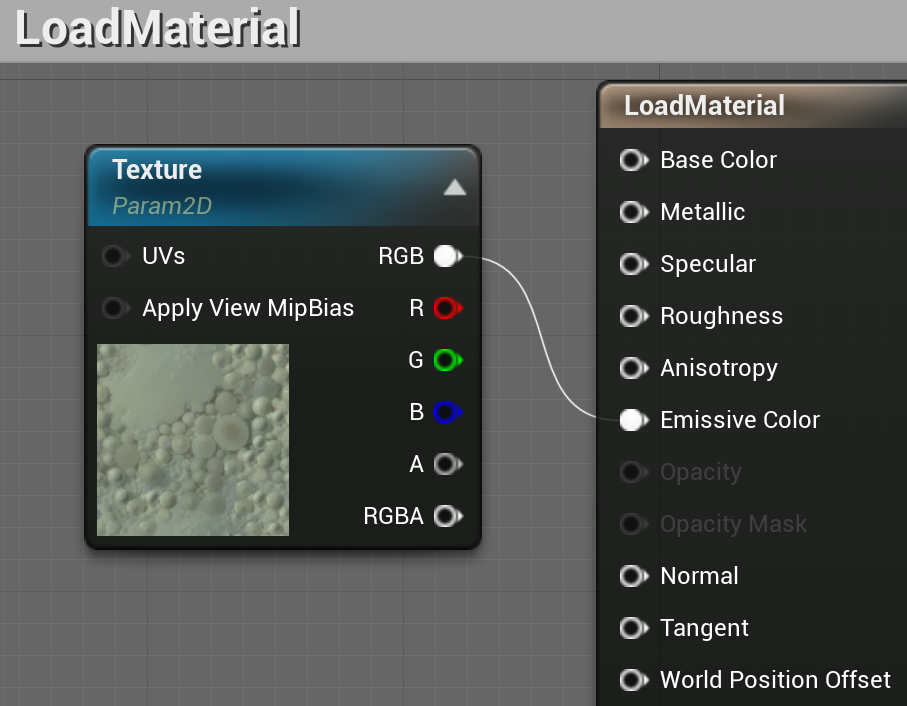
\includegraphics[width=0.8\textwidth]{img/load-material.png}
    \caption[Unreal Material used for loading.]{Unreal Material used for loading.~\cite{texture-loading-tutorial}}
    \label{fig:load-material}
\end{figure}
